\documentclass[handout,notes=show]{beamer}
%\documentclass[handout,notes=show]{beamer}
\usepackage{pgfpages}
%\pgfpagesuselayout{4 on 1}[letterpaper,landscape, border shrink=5mm]

%\documentclass{beamer}
\usepackage{epstopdf}
\usepackage{amsfonts}
\usepackage{amssymb}
\usepackage{amsmath}

\usepackage{subfig}



\newcommand{\vk}{\ensuremath{\mathbf{k}}}
\newcommand{\vK}{\ensuremath{\mathbf{K}}}
\providecommand{\vr}{\ensuremath{\mathbf{r}}}
%\newcommand{\vec}[1]{\ensuremath{\mathbf{#1}}}

\newcommand{\gk}{\ensuremath{{g}(\mathbf{k})}}

\newcommand{\vp}{\ensuremath{\mathbf{p}}}
\newcommand{\gp}{\ensuremath{{g}(\mathbf{p})}}

\newcommand{\vq}{\ensuremath{\mathbf{q}}}

\newcommand{\Fo}{\ensuremath{\mathbf{F_0}}}


\newcommand{\E}{\ensuremath{\mathbf{E}}}
\newcommand{\A}{\ensuremath{\mathbf{A}}}
\newcommand{\J}{\ensuremath{\mathcal{J}}}

\newcommand{\ket}[1]{\ensuremath{\left|#1\right>}}
\newcommand{\bra}[1]{\ensuremath{\left<#1\right|}}

\newcommand{\twoe}{\ensuremath{2\epsilon_\vk-\E_1}}

\newcommand{\nth}[1]{\ensuremath{\frac{1}{#1}}}

\newcommand{\br}[1]{\ensuremath{\left(#1\right)}}
\newcommand{\mbr}[1]{\ensuremath{\left[#1\right]}}
\newcommand{\bbr}[1]{\ensuremath{\left\{#1\right\}}}


\newcommand{\tk}{\ensuremath{\tilde{k}}}

\newcommand{\kp}{\ensuremath{\ket{\Psi}}}

\newcommand{\av}[1]{\ensuremath{\bigl<{#1}\bigr>}}
\newcommand{\avs}[3] {\av{#1{\lvert{#2}\rvert}#3}}
\newcommand{\avv}[2][\nu] {\avs{#1}{#2}{#1}}
\newcommand{\avt}[2]{\av{{#1}|{#2}}}
\newcommand{\avtu}[1]{\av{T_\tau#1}}

\newcommand{\Bop}{\ensuremath{\mathbf{B_0^+}}}
\newcommand{\Bmp}{\ensuremath{\mathbf{B_m^+}}}
\newcommand{\Bnp}{\ensuremath{\mathbf{B_n^+}}}
\newcommand{\Bo}{\ensuremath{\mathbf{B_0}}}
\newcommand{\Bopn}{\ensuremath{\mathbf{{B_0^+}^n}}}
\newcommand{\Bon}{\ensuremath{\mathbf{{B_0}^n}}}


\newcommand{\zmatrix}{\ensuremath{\br{\begin{smallmatrix}0&0\\0&0\end{smallmatrix}}}}
\newcommand{\fmtrx}[4]{\ensuremath{\br{\begin{smallmatrix}#1&#2\\#3&#4\end{smallmatrix}}}}
\newcommand{\smtrx}[6]{\ensuremath{\br{\begin{smallmatrix}#1&#2\\#3&#4\\#5&#6\end{smallmatrix}}}}

\newcommand{\vz}{\ensuremath{v^{\beta\alpha}_{\vk,\vk}}}


\providecommand{\abs}[1]{\ensuremath{\lvert{#1}\rvert}}

\newcommand{\sg}[1][1]{\ensuremath{\sigma_\frac{#1}{2}}}

\newcommand{\rhof}{\ensuremath{\rho(\ef)}}
\newcommand{\omt}{\ensuremath{\tilde{\Omega}}}
\newcommand{\cht}{\ensuremath{\tilde{\chi_0}}}
\newcommand{\Atl}{\ensuremath{\abs{A}^{2l}}}
\newcommand{\ef}{\ensuremath{\epsilon_F}}

\newcommand{\lca}{\ensuremath{\ln\br{1+\frac{\cht}{\alpha}}}}

\newcommand{\com}[2]{\ensuremath{\mbr{#1,#2}}}
\newcommand{\D}{\ensuremath{\mathit{D}}}
\newcommand{\dg}{\ensuremath{\dagger}}
\newcommand{\nG}{\ensuremath{\hat{\mathcal{G}}^{-1}}}

\providecommand{\lvk}{\ensuremath{1/\vk_F}}
\providecommand{\hm}{\ensuremath{\frac{\hbar^2}}{2m}}
\providecommand{\pdiff}[2]{\ensuremath{\frac{\partial{#1}}{\partial{#2}}}}
\providecommand{\dpdiff}[2]{\ensuremath{\frac{\partial^2{#1}}{\partial{{#2}^2}}}}

\providecommand{\H}{\ensuremath{\mathcal{H}}}
\providecommand{\wt}[1]{\widetilde{#1}}

\providecommand{\eef}[1]{Eq. (\ref{#1})}

\providecommand{\sch}{{Schr\"{o}dinger }}

\providecommand{\sgn}{\ensuremath{\text{sgn}}}
\newcommand{\Arctg}{\ensuremath{\text{Arctg}}}

\providecommand{\comm}[1]{\textit{\scriptsize \uwave{(#1)}}}
\newcommand{\myemph}[1]{\textbf{\color{blue!100}#1}}
\newcommand{\mathemph}[1]{{\color{red}#1}}
% \usepackage{beamerthemesplit} // Activate for custom appearance

\title[Crossover w/ 3-species]{BEC-BCS Crossover with the Feshbach Resonance for a Three-Hyperfine-Species Model}
\author[Guojun Zhu]{Guojun Zhu}
\institute{University of Illinois at Urbana-Champaign}
\date{Dec. 15th, 2011}
\pgfdeclareimage[height=1cm]{university-logo}{uiucLogo2.jpg}
\logo{\pgfuseimage{university-logo}}
%\usetheme[language=english,
%titlepagelogo=logopolito, bullet=circle, pageofpages=of, titleline=true, color=blue
%]{TorinoTh}
%\rel{Anthony J. Leggett}
%\usetheme[hideothersubsections, width=2cm]{PaloAlto}
\usetheme[hideothersubsections]{Berkeley}

%\usetheme{Hannover}
\usecolortheme{sidebartab}
\usefonttheme[onlymath]{serif}
%\usecolortheme{lily}
\AtBeginSection[]
{
  \begin{frame}
    \frametitle{Table of Contents}
    \tableofcontents[currentsection]
  \end{frame}
}
\begin{document}

\frame{
%\frametitle{Dissertation}
\titlepage}

\section[Outline]{}
\frame{
\frametitle{Outline}
\tableofcontents
}

\section{Introduction}
%\frame
%{
%  \frametitle{Features of the Beamer Class}
%
%  \begin{itemize}
%  \item<1-> Normal LaTeX class.
%  \item<2-> Easy overlays.
%  \item<3-> No external programs needed.      
%  \end{itemize}
%}


\frame{
\frametitle{Problems}
\begin{itemize}[<+->]
\item General narrow vs broad
\item Three species, interchannel Pauli exclusion
\end{itemize}
}

\section[Atomic Ham.]{Dilute ultracold alkali gas}\label{sec:intro:one}
\frame{
\frametitle{Single atom interaction (in spins)}
Hamiltonian:
\begin{equation}
\begin{split}\label{eq:intro:1atom}
H_{spin}&=A \mathbf{I}\cdot\mathbf{S}-\mu_{e}\mathbf{B}\cdot\mathbf{S}-{\mu}_{n}\mathbf{B}\cdot\mathbf{I}\\
&=A \mathbf{I}\cdot\mathbf{S}-\mu_{e}{B}{S_{z}}-{\mu}_{n}{B}{I_{z}}
\end{split}
\end{equation}
\begin{itemize}[<+->]
\item Diagonized by total angular momentum at the  zero magnetic field $(F,F_{z})$ 
\begin{equation}
\mathbf{F}=\mathbf{S}+\mathbf{I}
\end{equation}

\item $(F,F_{z})$  are no longer eigenstate at a finite magnetic field. 

\end{itemize}
}
\frame{
\frametitle{Hyperfine spin levels for one \textsuperscript{6}Li atom}
\begin{figure}[htbp]
\begin{center}
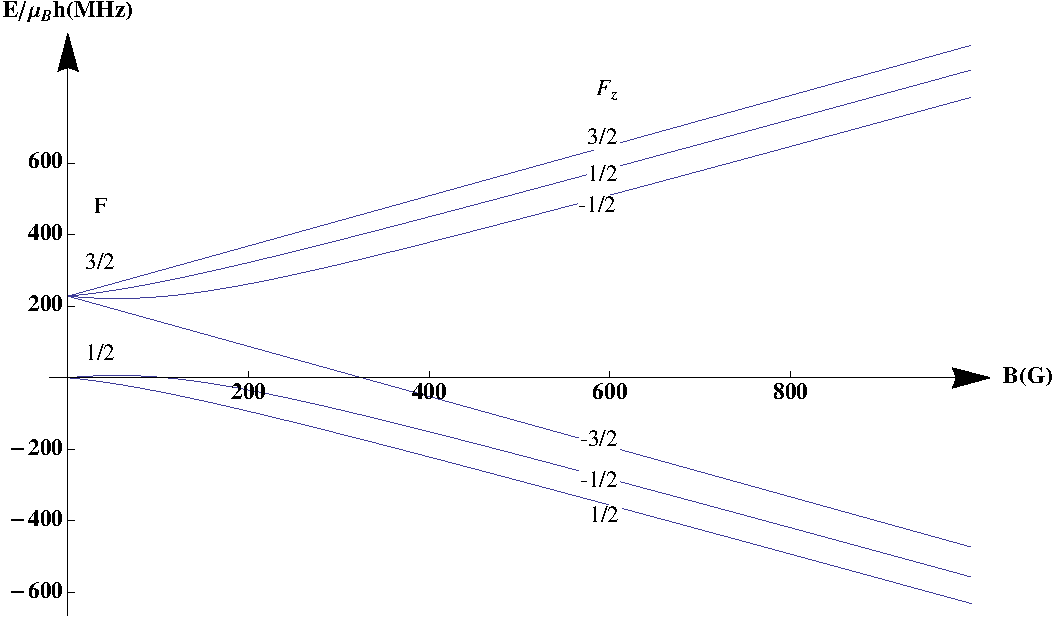
\includegraphics[width=0.8\textwidth]{hyperfineLi6}
\caption{Hyperfine structure of a  \textsuperscript{6}Li atom } 
%Levels are marked with $F$ and $F_{z}$ {(see Footnote \ref{foot:intro:f} in page \pageref{foot:intro:f})} %Note that the energy of the $\ket{F=\nth{2},F_z=-\nth{2}}$ state first increases with the magnetic field, $B$, at low field then decrease at high field. In the same way, the energy of the $\ket{F=\frac{3}{2},F_z=-\nth{2}}$ state first decreases and then increases with the magnetic field.  
\label{fig:intro:li6}
\end{center}
\end{figure}
}

\frame{
\frametitle{Interaction between two atoms}

\begin{itemize}[<+->]
\item Channels: one  configuration of hyperfine spins for one atom pair in interaction, $\ket{F^{(1)},F_{z}^{(1)}}\otimes\ket{F^{(2)},F_{z}^{(2)}}$ 
\item Interaction mostly due to electrons
\begin{equation}\label{eq:intro:two}
V=f(r)+g(r)\mathbf{S_{1}}\cdot\mathbf{S_{2}}
\end{equation}
\item Channels are mixed. 
\item In high field, channels are good zeroth approximation.
\item Resonances are possible. 
\end{itemize}
}
\subsection{Universality}
\frame{
\frametitle{S-wave scattering length, $a_s$}


 To describe low-energy phenomenon, a short-range potential can be characterized with a single parameter, $a_s$.
\begin{itemize}

\item Two domains: short-range, long-range (free range)
\item Bethe-Peierls boundary condition for long-range
\begin{equation}\label{eq:intro:Bethe}
\psi(r)\xrightarrow{r\to0}A\br{\nth{r}-\frac{1}{\mathemph{{a_s}}}}
\end{equation}
\item $a_s$ depends on \myemph{two-body}  physics only
\item $a_s$ coincides with the s-wave scattering length in for a scattering state

\item Valid in both positive and negative energy cases


\end{itemize}


}
\frame{
\frametitle{Universality}
\begin{equation}\tag{\ref{eq:intro:Bethe}}
\psi(r)\xrightarrow{r\to0}\mathemph{A}\br{\nth{r}-\nth{a_s}}
\end{equation}
The normalization $\mathemph{A}$ is determined by the \myemph{many-body} effects. 
\begin{itemize}
\item \emph{Integrated contact intensity}, $C$,  by Tan\cite{Tan2008-2}. $C\propto{A^2}$
\item Limit at high-momentum of the particle number distribution of particles, 
 \begin{equation}
 \lim_{k\to\infty}n_k=\frac{C}{k^4}
 \end{equation}

\end{itemize}
}
\frame{

\frametitle{Two-body density matrix}
Two body density matrices are important for fermion systems
 \begin{equation*}\label{eq:intro:2bodyDM}
 \av{\Psi^\dg(x_1)\Psi^\dg(x_2)\Psi(y_2)\Psi(y_1)}=\sum_nC_n\phi_n^\dg(x_1,x_2)\phi_n(y_1,y_2)
 \end{equation*}   
 \begin{itemize}
\item Quantum phenomena emerge when one or a few terms are macroscopic.
\item The eigen-functions with macroscopic eigenvalues are often called \myemph{order prarameters}.
\item The short-range part of the eigen-functions are proportional to the short-range of the two-body wave functions for the short-range potential at low-energy. 
\item The Bethe-Peierls boundary condition is the simplest non-trivial case (to the first order). 
\end{itemize}
}

 \section[2-body F.R.]{The  Feshbach resonance in two-body physics\label{sec:intro:twobody}}
 \frame{
 \frametitle{The Feshbach resonance in two-body physics}
 \begin{itemize}
\item  Two channels: open-channel and closed-channel 
\item Different electronic spins;  therefore different Zeeman energies
\item The uncoupled closed-channel would have a bound state with energy close to the threshold of the open-channel 
\item The low-energy effective scattering properties ($a_s$) in the open-channel is greatly modified.
\item $a_s$ is tunable by the magnetic field. 

\end{itemize}
 }
 
 \frame{
 \frametitle{Effective open-channel s-wave scattering length}
\begin{equation}
a_{s}(B)=a_{bg}\br{1+\frac{\Delta{B}}{B-B_{0}}}
\end{equation}
 \begin{figure}[htbp]
\begin{center}
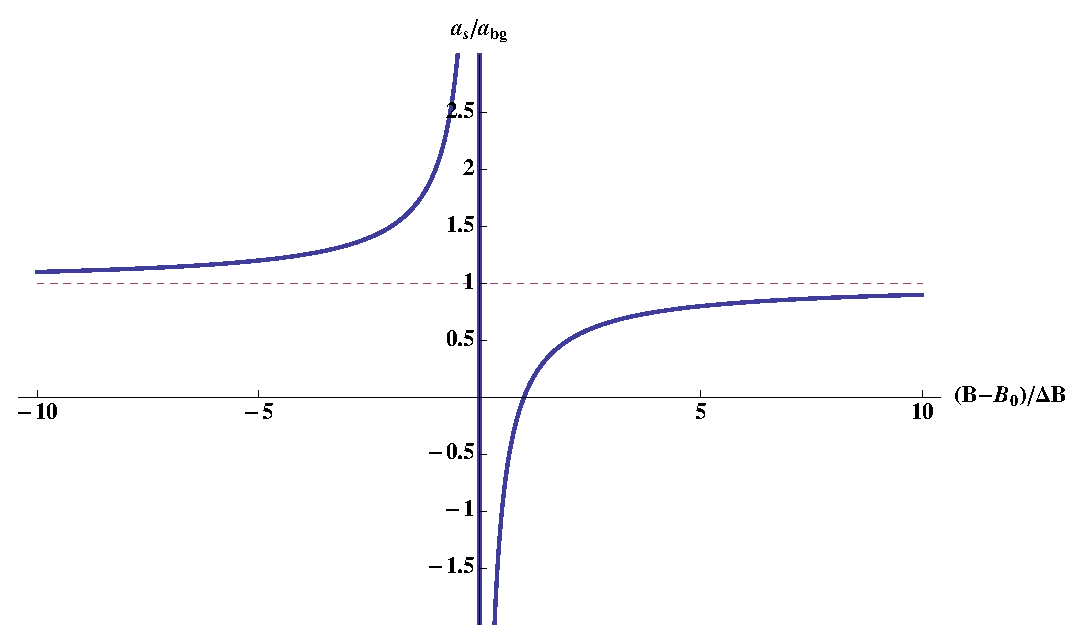
\includegraphics[width=0.8\textwidth]{FeshbachAs}
\caption{S-wave scattering length in Feshbach resonance} 
\label{fig:intro:Feshbach}

\end{center}
\end{figure}

 }
\frame{
\frametitle{Energy levels}
%\begin{columns}
%
%\begin{column}{0.6\textwidth}
\begin{figure}[htbp]
\begin{center}
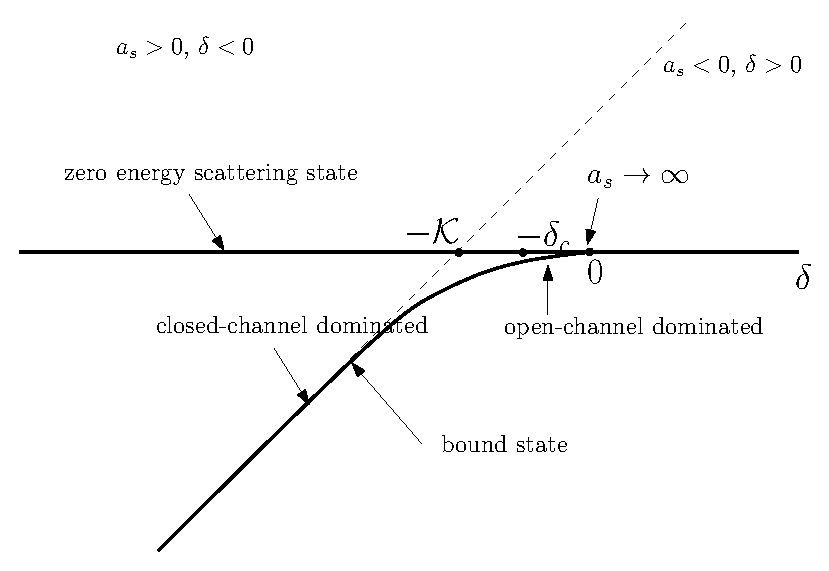
\includegraphics[width=0.9\textwidth]{levels}
\caption{Energy levels in a Feshbach resonance\label{fig:intro:levels}} 
%\parbox{0.9\textwidth}{\small $\delta$ is the energy detuning from the resonance point, where the resonant point is defined as the point where the open-channel effective s-wave scattering length diverges, $a_s\to\pm\infty$.  The horizontal line stands for the zero energy s-wave scattering state, $\psi\sim\nth{r}-\nth{a_s}$, which exists for any detuning.  The lower line stands for the real bound state, which only exists for negative detuning ($\delta<0$, $a_s>0$). The dash line stands for the (uncoupled) closed-channel bound state.  An interesting point to notice is that the real bound state appears earlier than the cross point of the (uncoupled) closed-channel bound state level and zero energy. Another important point to notice is the negative detuning $-\delta_c$.  When the negative detuning is smaller than $\delta_c$, this real bound state is composed mostly with atoms in the open-channel and vice verse.  See Chapter \ref{sec:intro:twobody} for details about $\mathcal{K}$ and $\delta_c$.   }

\end{center}
\end{figure}
%\end{column}
%\begin{column}{0.35\textwidth}

%\end{column}
%\end{columns}
}


\begin{frame}
\frametitle{Feshbach }
\begin{itemize}
\item Resonant point is not the level crossing point. The shift $\mathcal{K}$ is large than most energy scales. 
\item At negative detuning, a characteristic energy scale $\mathemph{\delta_c}$, $\lambda=n_{close}/n_{open}$ 

\end{itemize}
\begin{tabular}{|p{4cm}|p{4cm}|}
\hline
 $\mathemph{\abs{\delta}\ll\delta_{c}}$&$\mathemph{\abs{\delta}\gg\delta_{c}}$\\\hline
 $\abs{E}\approx\delta^{2}/\delta_{c}\ll\abs{\delta}$&$E\approx\delta$\\\hline $\lambda\approx{\delta/(\sqrt{2}\delta_{c})}\ll1$& 
 $\lambda=\sqrt{|\delta|/(2\delta_{c})}\gg1$\\\hline
 Atoms are predominantly in the closed-channel.&Atoms are predominantly in the closed-channel.\\
 \hline
\end{tabular}
\end{frame}

\begin{frame}
        \frametitle{Broad resonance}
        Comparing $\delta_c$ with the many-body scale, $E_F$
 
       $\mathemph{\delta_c\gg{}E_F}$
        \begin{itemize}

\item The closed channel weight is negligible everywhere in the crossover.
\item The closed channel is just like a simple knob for the effective open-channel interaction
\item The single-channel models' solutions are directly applied.
\end{itemize}
   
\end{frame}

\begin{frame}
        \frametitle{Narrow resonance}
        
 
       $\mathemph{\delta_c\ll{}E_F}$
        \begin{itemize}

\item The closed channel weight is substantial or even dominant close to the resonance.
\item Both channels need to be considered in the many-body framework. 
\item One simplification: the uncoupled closed-channel bound state is much smaller than the interparticle distance. 
\end{itemize}
\end{frame}


\section[Single-channel]{Single-channel BEC-BCS crossover}   



\frame{
\frametitle{Model setup}
Action and partition function
\begin{gather}\label{eq:pathInt2:actionPsi}
\begin{split}
&S[\bar\psi,\psi]\\=&\int^{\beta}_{0}d\tau\int{d^{d}\vr}\Big[\sum_{\sigma}\bar\psi_{\sigma}(\vr,\tau)\br{\partial_{\tau}-\nth{2m}\nabla^{2}-\mu}\psi_{\sigma}(\vr,\tau)\\&-g\bar\psi_{\uparrow}(\vr,\tau)\bar\psi_{\downarrow}(\vr,\tau)\psi^{}_{\downarrow}(\vr,\tau)\psi^{}_{\uparrow}(\vr,\tau)\Big]
\end{split}\\
\mathcal{Z}=\int{\bigD(\bar\psi,\psi)\exp\br{-S[\bar\psi,\psi]}}
\end{gather}
Note that here we use the contact interaction.  
}
\frame{
\frametitle{Hubbard-Stratonovich transformation}
We introduce an auxiliary field (functional variable) $\Delta(\vr,\tau)$ coupled with a pair $\psi_{\uparrow}(\vr,\tau)\psi_{\downarrow}(\vr,\tau)$. 

\begin{equation*}\label{eq:pathInt:expHS}
\begin{split}
&\exp\br{g\int{d\tau{}d^{d}\vr}\bar{\psi}_{\uparrow}\bar\psi_{\downarrow}\psi_{\downarrow}\psi_{\uparrow}}=\\
&\int{\bigD(\bar\Delta,\Delta)}\exp\bbr{-\int{d\tau{d^{d}\vr}}\mbr{\nth{g}{\bar\Delta}{\Delta}-\br{\bar\Delta\psi_{\downarrow}\psi_{\uparrow}+\Delta\bar\psi_{\uparrow}\bar\psi_{\downarrow}}}}
\end{split}
\end{equation*}
\begin{itemize}
\item Exact mathematical identity, variation of Gaussian integral
\item Remove the four-variable coupling
\item Introduce an auxiliary field

\end{itemize}
}

\frame{
\frametitle{Hubbard-Stratonovich transformation (2)}
Introduce Nambu representation,
\begin{equation}
\bar\Psi=\begin{pmatrix}\bar{\psi}_{\uparrow}&\psi_{\downarrow}\end{pmatrix}\text{,  }\qquad
\Psi=\begin{pmatrix}{\psi}_{\uparrow}\\\bar\psi_{\downarrow}\end{pmatrix}
\end{equation}
The partition function with $\Delta$
\begin{equation*}\label{eq:pathInt:ZDeltaPhi}
\mathcal{Z}=\iint{\bigD(\bar\Psi,\Psi,\bar\Delta,\Delta)}\exp
	\bbr{-\int{d\tau{d^{d}\vr}}\mbr{\nth{g}{\bar\Delta}{\Delta}-\bar\Psi \nG\Psi}}
\end{equation*}
where the Gor'kov Green function is
\begin{equation*}\label{eq:pathInt:nG}
\nG=\begin{pmatrix}
[\hat{G}_{0}^{(p)}]^{-1}&\Delta\\\bar\Delta&[\hat{G}_{0}^{(h)}]^{-1}
\end{pmatrix}
\end{equation*}
 $[\hat{G}_{0}^{(p)}]^{-1}=-\partial_{\tau}+\nth{2m}\nabla^{2}+\mu$,  $[\hat{G}_{0}^{(h)}]^{-1}=-\partial_{\tau}-\nth{2m}\nabla^{2}-\mu$ 

}

\frame{
\frametitle{Hubbard-Stratonovich transformation (3)}
The partition function of only $\Delta$
\begin{equation}\label{eq:pathInt:DeltaPF}
\mathcal{Z}=\int{\bigD(\bar\Delta,\Delta)}\exp
	\bbr{-\mbr{\br{\int{d\tau{d^{d}r}}\nth{g}{\bar\Delta\Delta}}-\mathemph{\ln\det\nG}}}
\end{equation}
\begin{itemize}
\item The $\mathemph{\ln\det\nG}$ term is highly non-trivial and contains all the many-body physics
\item Exact result so far.  Approximation starts when we take the mean-field result. 
\end{itemize}
}
\subsection{Mean-field result}
\begin{frame}
\frametitle{Gap equation}
Find the saddle point,   differentiate last equation with respect to $\Delta$
\begin{equation*}
\nth{g}\bar{\Delta}(\vr,\tau)-\tr\mbr{\hat{\mathcal{G}}(\vr,\tau,\vr,\tau)\begin{pmatrix}0&1\\0&0\end{pmatrix}}=0
\end{equation*}
take $\Delta$ as spacial-tempo uniform, $\Delta_{0}$
\begin{equation*}
\nth{g}\bar{\Delta}_0=\frac{T}{\mathcal{V}_{0}}\sum_{\vp,n}\frac{\bar\Delta_0}{\omega_n^2+E_\vp^2}
\end{equation*}
sum the Matsubara frequency 
\begin{equation}
\nth{g}=\nth{\mathcal{V}_{0}}\sum_{\vp}\frac{\tanh{(E_p/2T)}}{2E_p}
\label{eq:pathInt:gap}
\end{equation}
\end{frame}

\frame{
\frametitle{Renormalization of the gap equation}

\begin{equation}
\nth{g}=\nth{\mathcal{V}_{0}}\sum_{\vp}\frac{\tanh{(E_p/2T)}}{2E_p}
\tag{\ref{eq:pathInt:gap}}
\end{equation}
The summation in the gap equation diverges for 3D because the artificial assumption of the contact interaction. Considering a similar divergence in two-body scattering problem
\begin{equation*}\label{eq:pathInt:as}
\frac{m\mathcal{V}_{0}}{4\pi{}a_{s}}=-\nth{g}+\sum_{k<\Lambda}\nth{2\epsilon_{\vk}}
\end{equation*}
We derived \myemph{the renormalized gap equation}
\begin{equation}\label{eq:pathInt:gapRenormalized}
\boxed{-\frac{m\mathcal{V}_{0}}{4\pi{}a_{s}}=\sum_{\vk}\mbr{\frac{\tanh{(E_k/2T)}}{2E_k}-\nth{2\epsilon_{\vk}}}}
\end{equation}
}

\frame{
\frametitle{Number equation}
To complement the gap equation, we have the number equation
\begin{equation*}
N=-\nth{\beta}\tr\br{{G_{0}\pdiff{G_{0}^{-1}}{\mu}}}
\end{equation*}
Similarly the summation (due to the trace) over the Mastubara frequency can be evaluated and we have the number equation
\begin{equation}
\boxed{N=\nth{L^{d}}\sum_{\vk}\mbr{1-\frac{\epsilon_{\vk}}{E_{\vk}}\tanh{(\frac{E_{\vk}}{2T})}}}
\end{equation}

}


\frame{
\frametitle{$\mu$ and $\Delta$ in the crossover}
\begin{figure}[htbp]
\begin{center}
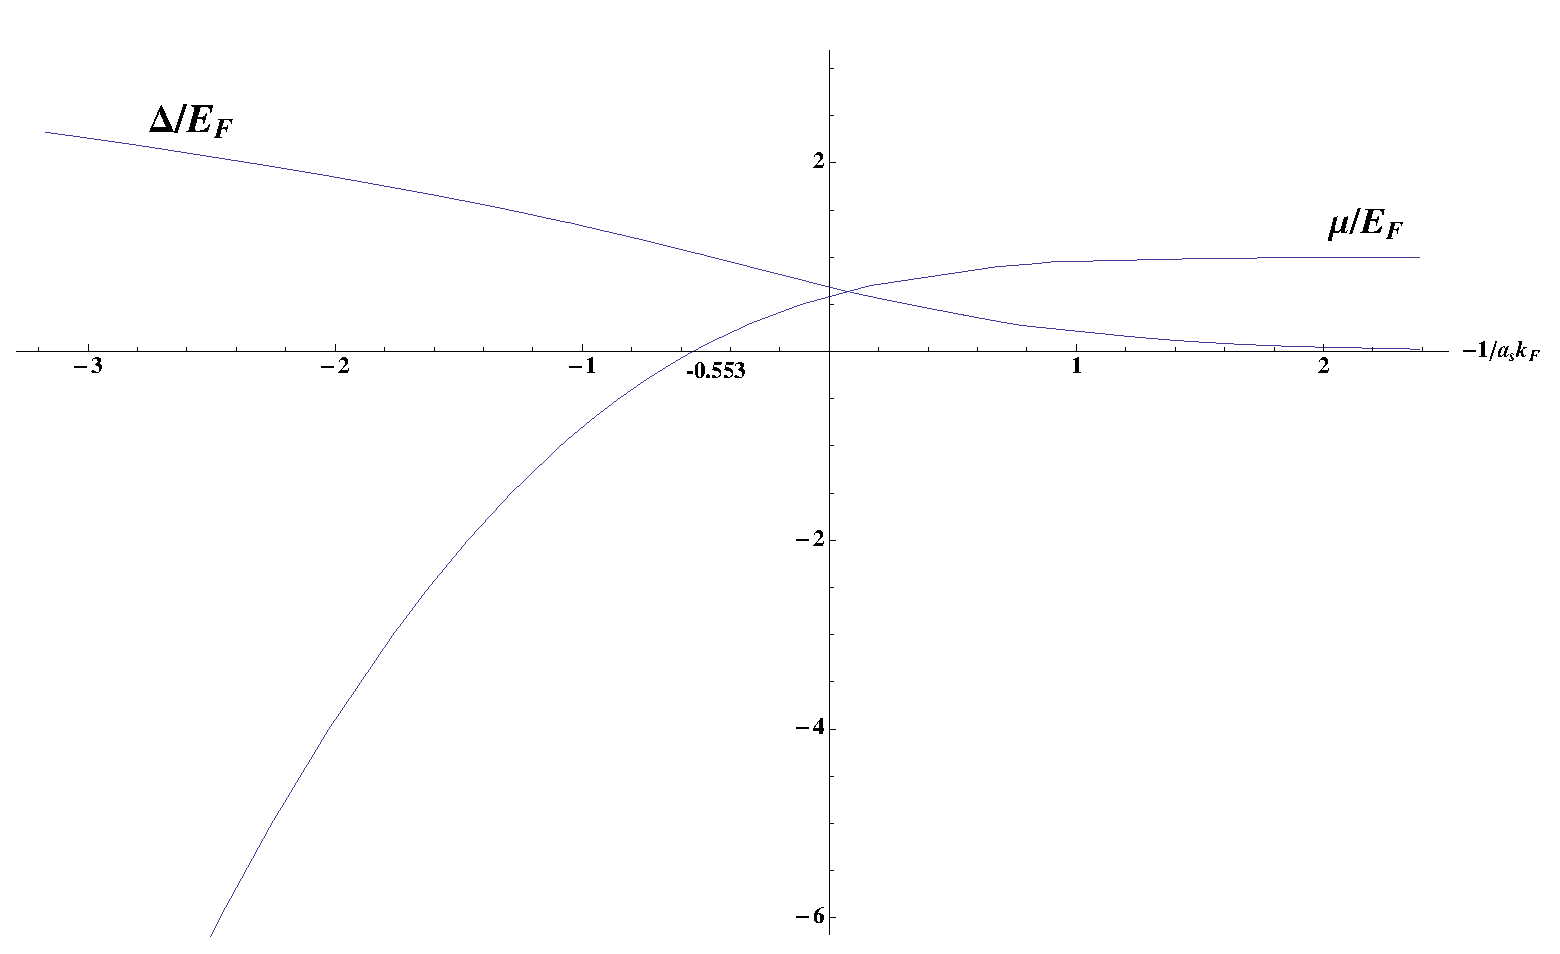
\includegraphics[width=0.8\textwidth]{SingleChannelCrossoverMuDelta}
\caption{The chemical potential $\mu$ and gap $\Delta$ in the mean field level over crossover} 
\label{fig:pathInt:meanField}
{\small All quantities in the unit of energy ($\mu$, $\Delta$) are rescaled with the Fermi energy $E_{F}$ and the s-wave scattering length $a_{s}$ is rescaled with $1/k_{F}$.  }
\end{center}
\end{figure}
}

\subsection[excitation]{Excitation modes}
\frame{
\frametitle{Fermionic excitation modes and the Bogoliubov transformation}
Gor'kov Green function in the momentum-frequency repensentation
\begin{equation}
\nG=\mtrx{i\omega_{n}-\xi_{k}&\Delta\\\bar\Delta&i\omega_{n}+\xi_{k}}=T^{\dg}BT
\end{equation}
\begin{equation}
T=\mtrx{u_{k}&v_{k}\\-v_{k}^{*}&u_{k}}\qquad{}B=\mtrx{i\omega_{n}+E_{k}&0\\0&i\omega_{n}-E_{k}}
\end{equation}
\begin{itemize}
\item $T$ is the Bogoliubov canonical transformation
\item Two excitation modes are \myemph{gapped}, $E_{k}=\sqrt{\xi^{2}_{\vk}+\Delta^{2}}$. 
\item One of them ($-E_{\vk}$) has an extra negative sign because it corresponds to $\psi\bar\psi=-\bar\psi\psi$.
\end{itemize}
}

\frame{
\frametitle{Anderson-Bogoliubov collective mode}
Expand the order parameter around the saddle point, $\Delta(\vr,\tau)=\Delta_{0}+\theta(\vr,\tau)$, we derived the action as
\begin{equation}
S[\Delta_{0},\theta,\theta^{*}]=S[\Delta_{0}]+\nth{2}\sum_{q}\mbr{\theta^{\dg}(q)\mathbf{M}(q)\theta(q)}
\end{equation}
\begin{equation*}
\begin{split}
&\mathbf{M}(q)=\\
&\begin{pmatrix}
\nth{g}+\sum_{p}G_{0}{\ }_{11}(p)G_{0}{\ }_{22}(p-q)&\sum_{p}G_{0}{\ }_{12}(p)G_{0}{\ }_{12}(p-q)\\
\sum_{p}G_{0}{\ }_{12}(p)G_{0}{\ }_{12}(p-q)&\nth{g}+\sum_{p}G_{0}{\ }_{11}(p-q)G_{0}{\ }_{22}(p)
\end{pmatrix}
\end{split}
\end{equation*}

}


\frame{
\frametitle{Anderson-Bogoliubov collective mode (2)}
Looking for roots of $\abs{M(\omega,\vq)}=0$. Only looking for roots with small momentum, $\vq$, and frequency, $\omega$, ($\omega\ll\Delta$, $\hbar^{2}\vq^{2}/2m\ll\Delta$). We find a sound wave
\begin{equation}
\omega\approx{}c\,q
\end{equation}
\begin{itemize}
\item  At the BCS side, $c=v_{F}/\sqrt{3}$. 
\item At the BEC side, we get $c^{2}=\Delta^{2}/8m\abs{\mu}=4\pi{}n_{B}a_{B}/m_{B}$.  This leads to  $a_{B}=2a_{s}$ as the effective interaction strength between two-atom dimmers.  This deviates from more accurate calculation, $a_{B}=0.6a_{s}$ \cite{Petrov}, which indicates the possible deficiency of the current theory. 

\end{itemize}
}
%
\section[Mean-feild]{Mean-field result of the two-channel models}

\frame{
\frametitle{Extremely narrow resonance}
The coupling between two channels is assumed to be extremely weak. $\delta_{c}\to0$. Two channels share the same chemical potentials. 
\begin{figure}[hhtb]
	\centering
	         \subfloat[$E_{F}<\tilde\delta$]{\label{fig:narrowFR:aboveSea}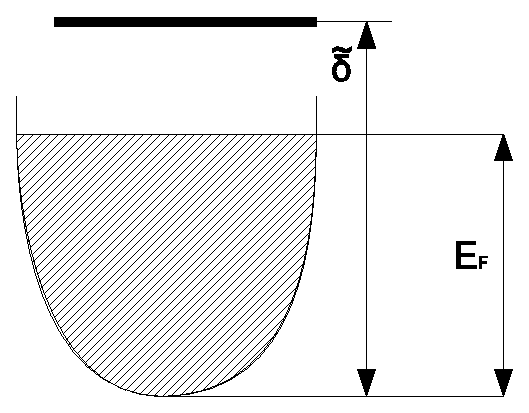
\includegraphics[width=.2\textwidth]{narrowFRabove.eps}}\quad
		\subfloat[$0<\tilde\delta<E_{F}$]{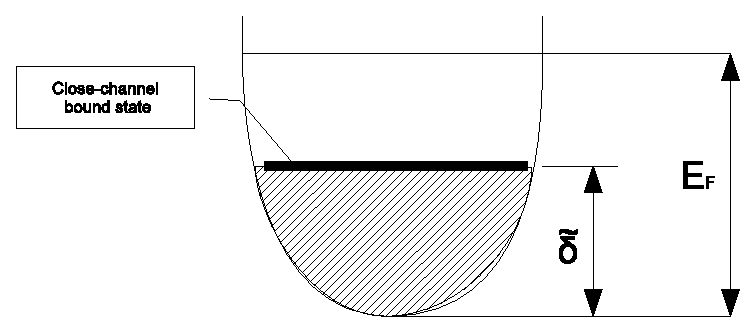
\includegraphics[width=.30\textwidth]{narrowFRin.eps}\label{fig:narrowFR:inSea}}\quad
		\subfloat[$\tilde\delta<0$]{\label{fig:narrowFR:belowSea}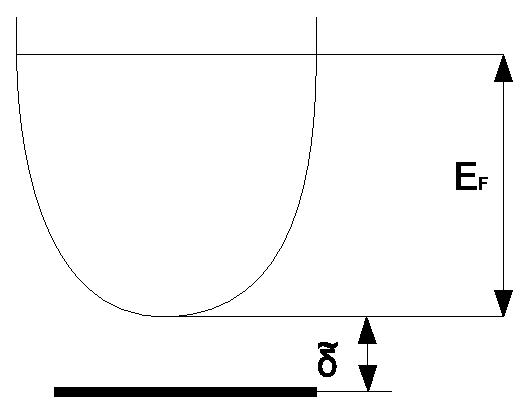
\includegraphics[width=.20\textwidth]{narrowFRbelow.eps}}
	\caption{Extremely narrow resonance\label{fig:narrowFR}}
	\small{The shaded area is occupied by atoms. }
	%\parbox{0.7\textwidth}{\small{  In Fig. \subref{fig:narrowFR:inSea} chemical potential would be close to the closed-channel bound state level (besides small shift due to the open-channel intra-channel coupling) and the ``Fermi sea'' above is empty. }}
\end{figure}
}



\frame{
\frametitle{Model setup}


The finite-temperature action is 
\begin{equation}
\begin{split}\label{eq:pathInt2:actionFermi}
&S(\bar\psi,\psi)=\int^{\beta}_{0}d\tau\int{d^{d}r}\\
&\Big[\sum_{j}\bar\psi_{j}(\partial_\tau-\nth{2m}\nabla^{2}-\mu+\eta_{j})\psi_{j}
-(\bar\psi\bar\psi)\tilde{U}(\psi\psi)\Big]
\end{split}
\end{equation}
$\eta_{j}$ is the Zeeman energy of the hyperfine species j. Two channels are expressed as a 2-component vector
\begin{equation*}
(\bar\psi\bar\psi)=\mtrx{\bar\psi_{a}\bar\psi_{b}&\bar\psi_{a}\bar\psi_{c}}
\qquad(\psi\psi)=\mtrx{\psi_{b}\psi_{a}\\\psi_{c}\psi_{a}}
\end{equation*}
We have \myemph{contact} interaction 
\begin{equation}
\tilde{U}\equiv{}\mtrx{U&Y\\Y^{*}&V}
\end{equation}



}

\frame{
\frametitle{Hubbard-Stratonovich transformation}
Introduce a two-component auxiliary field
\begin{equation*}
\mtrx{\Delta_{1}\\\Delta_{2}}\longrightarrow
	\mtrx{\Delta_{1}\\\Delta_{2}}-
	\mtrx{U&Y\\Y^{*}&V}
	\mtrx{\psi_{b}\psi_{a}\\\psi_{c}\psi_{a}}
\end{equation*}
This coupling has built-in channel mixture. 

\begin{gather*}
\exp[\int{dx}(\bar\psi\bar\psi)\tilde{U}(\psi\psi)]\\
=\int{\bigD(\Delta,\bar\Delta)}\exp\big\{-\int{dx}
	[\Delta^{\dg}\tilde{U}^{-1}\Delta-(\bar\psi\bar\psi)\Delta-\bar\Delta{}(\psi\psi)]\big\}
\end{gather*}
}

\frame{
\frametitle{Hubbard-Stratonovich transformation (2)}
Introduce  a 3-component spinor similar to the Nambu spinor representation in the single-channel superconductivity.  
\begin{equation}
\bar\Psi=\mtrx{\bar\psi_{a}&\psi_{b}&\psi_{c}}\qquad\Psi=\mtrx{\psi_{a}\\\bar\psi_{b}\\\bar\psi_{c}}
\end{equation}
The action can then be rewritten in a more compact form with respect to $\Psi$ and $\bar\Psi$
\begin{equation}\label{eq:pathInt2:actionMixCompact}
S(\bar\Delta,\Delta,\bar\psi_{i},\psi_{i})=\int^{\beta}_{0}d\tau\int{d^{d}r}
	\mbr{\Delta^{\dg}\tilde{U}^{-1}\Delta-\bar\Psi\mathcal{G}^{-1}\Psi}
\end{equation}
It is bilinear of $\Psi$.  We can integrate it out,
\begin{equation}\label{eq:pathInt2:actionD}
S(\bar{\Delta},\Delta)=\int{dx}\br{\bar{\Delta}\tilde{U}^{-1}\Delta-\tr\ln\nG}
\end{equation}

}

\note{\begin{itemize}
\item This is different from the two-component channel-based vector.
\item For b,c, $\bar\psi$ and $\psi$ are reversed, which gives an extra negative sign.
�
\end{itemize}
}

\frame{
\frametitle{Gor'kov Green function}
where 
\begin{equation}
\mathcal{G}^{-1}=
\begin{pmatrix}\label{eq:pathInt2:nGDelta}
[\hat{G}_{0}^{(p)}]^{-1}-\eta_{a}&\Delta_{1}&\Delta_{2}\\
\bar\Delta_{1}&[\hat{G}_{0}^{(h)}]^{-1}+\eta_{b}&0\\
\bar\Delta_{2}&0&[\hat{G}_{0}^{(h)}]^{-1}+\eta_{c}
\end{pmatrix}
\end{equation}
 $[\hat{G}_{0}^{(p)}]^{-1}=-\partial_{\tau}+\nth{2m}\nabla^{2}+\mu$,  $[\hat{G}_{0}^{(h)}]^{-1}=-\partial_{\tau}-\nth{2m}\nabla^{2}-\mu$ 
Decoupled in the momentum-frequency space
\begin{equation*}\label{eq:pathInt2:nGDeltaK}
\mathcal{G}^{-1}=
\begin{pmatrix}
i\omega_{n}-\xi_{k}-\eta_{a}&\Delta_{1}&\Delta_{2}\\
\bar\Delta_{1}&i\omega_{n}+\xi_{k}+\eta_{b}&0\\
\bar\Delta_{2}&0&i\omega_{n}+\xi_{k}+\eta_{c}
\end{pmatrix}
\end{equation*}
$\xi_{k}=\nth{2m}k^{2}-\mu$
}
\frame{
\frametitle{Diagonalization of the Green's function\label{sec:diagonalGreen}}

\begin{equation}\label{eq:pathInt2:nG}
\mathcal{G}^{-1}=i\omega_{n}I-
\begin{pmatrix}
\xi_{k}&-\Delta_{1}&-\Delta_{2}\\
-\bar{\Delta}_{1}&-\xi_{k}&0\\
-\bar{\Delta}_{2}&0&-(\xi_{k}+\eta)
\end{pmatrix}
\end{equation}
\begin{itemize}
\item
Decoupled in the momentum-frequency space
\item Only need to be diagonalized in the $3\times3$ hyperfine-spin space
\end{itemize}
}

\frame{
\frametitle{Diagonalization of the Green's function (2)}
\begin{equation}\label{eq:pathInt2:B}
B_{\omega_{n},\vk}=L_k^{\dg}T_k^{\dg}G_{\omega_{n},\vk}^{-1}T_kL_k
\end{equation} 
\begin{equation}\label{eq:pathInt2:T}
T_k=\mtrx{u_k&v_k&0\\-v_k&u_k&0\\0&0&1}
\end{equation}	
\begin{gather*}
v_{\vk}^{2}\equiv1-u_{\vk}^{2}\equiv\nth{2}\br{1-\frac{\xi_{\vk}}{E_{\vk}}}\qquad
E_{\vk}\equiv(\xi_{\vk}^{2}+\Delta_{1}^{2})^{1/2}
\end{gather*}
$T_{k}$ is enough to diagonalize the $G$ matrix in the broad resonance case. 
}
\frame{
\frametitle{Diagonalization of the Green's function (3)}
For the narrow resonance,
\begin{equation}\label{eq:pathInt2:Bapprox}
B_{\omega_{n},\vk}=i\omega_{n}I-
	\mtrx{E_{1}{}_{\vk}&0&0\\0&-E_{2}{}_{\vk}&0\\0&0&-E_{3}{}_{\vk}}
%	&\approx{}i\omega_{n}I-
%	\mtrx{E_{\vk}+{}u_{\vk}^{2}\zeta&0&0\\
%	0&-\br{E_{\vk}-{}v_{\vk}^{2}\zeta}&0\\0&0&-\br{\xi_{\vk}+\eta-\frac{\zeta}{2}}}
%	&=
%	\mtrx{i\omega_{n}-E_{\vk}&0&0\\0&i\omega_{n}+E_{\vk}&0\\0&0&i\omega_{n}+\eta}
%	+\mtrx{-\frac{D_{1}^{2}}{\eta}&0&0\\0&-\frac{D_{2}^{2}}{\eta}&0\\0&0&+\frac{D_{1}^{2}+D_{2}^{2}}{2\eta}}\\
%	&\equiv{}B^{(0)}_{\vk}+B^{(1)}_{\vk}
\end{equation}
\begin{columns}
\column{0.7\textwidth}
\begin{align*}
E_{1\vk}&\approx{}E_{\vk}+u_{\vk}^{2}\Delta_{1}\zeta\\
E_{2\vk}&\approx{}E_{\vk}-v_{\vk}^{2}\Delta_{1}\zeta\\
E_{3\vk}&\approx{}\epsilon_{\vk}+\eta+\frac{\zeta}{2}\Delta_{1}
\end{align*}
\column{0.3\textwidth}
\begin{equation}\label{eq:pathInt2:zetaDef}
\boxed{\zeta=\frac{\Delta_{2}^{2}}{\Delta_{1}\eta}}
\end{equation}
\end{columns}
\begin{itemize}
\item The correction is in the order of $\zeta\ll1$
\item The correction is due to the inter-channel Pauli exclusion and does not disappear when there is no coupling. 
\end{itemize}
}

\frame{
\begin{equation}\label{eq:pathInt2:L1}
L_{\vk}\approx{}I+
\mtrx{0&-\frac{\Delta_{1}{}\Delta_{2}{}}{4E^{2}_{\vk}}&u_{\vk}\\
\frac{\Delta_{1}{}\Delta_{2}{}}{4E^{2}_{\vk}}&0&v_{\vk}\\
-u_{\vk}&-v_{\vk}&0
}\frac{\Delta_{2}{}}{\eta}
\end{equation}
\begin{itemize}
\item $L$ is not an identity only in the narrow resonance.  
\item $L$ is unitary only up to the first order of $\zeta$.
\end{itemize}
}



\frame{
	\frametitle{Narrow resonance w/o interchannel exclusion}
	\begin{itemize}
\item Energy zero moves to the Fermi surface
\begin{gather}
1=-\mbr{\frac{4\pi{\tilde{a}_{s}(\mu)}}{m}\sum(\nth{2E_{\vk}}-\nth{2\epsilon_{\vk}})}\label{eq:pathInt2:narrowGapS}\\
\tilde{a}_{s}=a_{\text{bg}}(1+\frac{\mathcal{K}}{\delta-2\mu})\approx{}\frac{a_{\text{bg}}\mathcal{K}}{\delta-2\mu}
\end{gather}
\item Extra counting for the closed-channel. 
\begin{gather}
N_{\text{open}}=\sum_\vk\frac{E_\vk-\xi_\vk}{2E_\vk}\label{eq:pathInt2:narrowNumS}
\end{gather}
\end{itemize}

}


\frame{
\frametitle{Narrow resonance w/o interchannel exclusion}
\begin{figure}[htbp]
\begin{center}
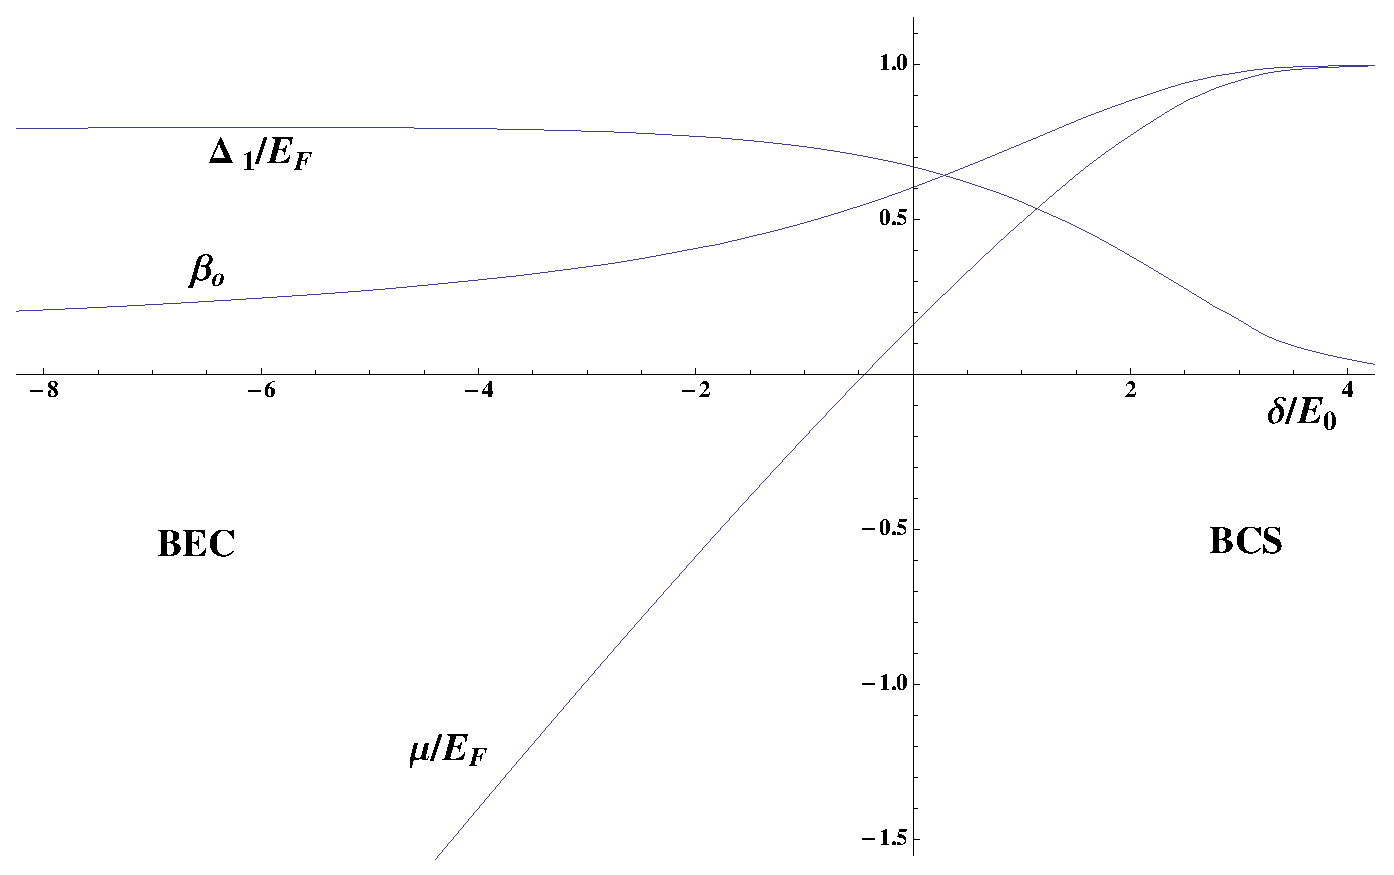
\includegraphics[width=0.8\textwidth]{narrow}
\caption{The chemical potential $\mu$, the open-channel gap $\Delta_{1}$ and the open-channel relative weight $\beta_{o}$ over crossover with the narrow Feshbach resonance without considering the inter-channel Pauli exclusion  vs. the chemical potential and the gap in the single-channel model} 
\label{fig:pathInt2:narrow}
{\small  The gap in the open-channel $\Delta_{1}$ and the chemical potential $\mu$ are rescaled with the the Fermi energy of the total density, $E_{F}^{(tot)}$.  The $x$-axis is the detuning $\delta$ rescaled with $E_{0}$ (see Eq. \ref{eq:pathInt2:E0}) for the narrow resonance; while it is $-1/a_{s}k_{F}$ for the single-channel curves. We have taken $\delta_{c}=0.001E_{F}^{(tot)}$ for the narrow resonance figure. We used the detuning from the resonant point  for the $x$-axis in the narrow resonance instead of $-1/a_{s}k_{F}$ in the single-channel because the additional shift, $2\mu$, considering in Eq. \ref{eq:pathInt2:simplenarrowAs}.  Consequently, the chemical potential lines in both cases cross the $x$-axis at the same point where $\mu=0$.  }
\end{center}
\end{figure}
}
\section[Excitation]{Excitation Mode}
\frame{
\frametitle{Fermionic modes and Bogoliubov transformation}
}
\frame{
\frametitle{Bosonic modes}
\begin{itemize}
\item Fluctuations of the order parameters;
\item Four possible modes for two complex order parameters ($\Delta_1$, $\Delta_2$);
\item The overall phase fluctuation mode is the Goldstone mode;
\item The other three modes are massive.

\end{itemize}
}

%\documentclass[]{beamer}
%t\documentclass[handout,notes=show]{beamer}
\usepackage{pgfpages}
%\pgfpagesuselayout{4 on 1}[letterpaper,landscape, border shrink=5mm]

%\documentclass{beamer}
\usepackage{epstopdf}
\usepackage{amsfonts}
\usepackage{amssymb}
\usepackage{amsmath}

\usepackage{subfig}



\newcommand{\vk}{\ensuremath{\mathbf{k}}}
\newcommand{\vK}{\ensuremath{\mathbf{K}}}
\providecommand{\vr}{\ensuremath{\mathbf{r}}}
%\newcommand{\vec}[1]{\ensuremath{\mathbf{#1}}}

\newcommand{\gk}{\ensuremath{{g}(\mathbf{k})}}

\newcommand{\vp}{\ensuremath{\mathbf{p}}}
\newcommand{\gp}{\ensuremath{{g}(\mathbf{p})}}

\newcommand{\vq}{\ensuremath{\mathbf{q}}}

\newcommand{\Fo}{\ensuremath{\mathbf{F_0}}}


\newcommand{\E}{\ensuremath{\mathbf{E}}}
\newcommand{\A}{\ensuremath{\mathbf{A}}}
\newcommand{\J}{\ensuremath{\mathcal{J}}}

\newcommand{\ket}[1]{\ensuremath{\left|#1\right>}}
\newcommand{\bra}[1]{\ensuremath{\left<#1\right|}}

\newcommand{\twoe}{\ensuremath{2\epsilon_\vk-\E_1}}

\newcommand{\nth}[1]{\ensuremath{\frac{1}{#1}}}

\newcommand{\br}[1]{\ensuremath{\left(#1\right)}}
\newcommand{\mbr}[1]{\ensuremath{\left[#1\right]}}
\newcommand{\bbr}[1]{\ensuremath{\left\{#1\right\}}}


\newcommand{\tk}{\ensuremath{\tilde{k}}}

\newcommand{\kp}{\ensuremath{\ket{\Psi}}}

\newcommand{\av}[1]{\ensuremath{\bigl<{#1}\bigr>}}
\newcommand{\avs}[3] {\av{#1{\lvert{#2}\rvert}#3}}
\newcommand{\avv}[2][\nu] {\avs{#1}{#2}{#1}}
\newcommand{\avt}[2]{\av{{#1}|{#2}}}
\newcommand{\avtu}[1]{\av{T_\tau#1}}

\newcommand{\Bop}{\ensuremath{\mathbf{B_0^+}}}
\newcommand{\Bmp}{\ensuremath{\mathbf{B_m^+}}}
\newcommand{\Bnp}{\ensuremath{\mathbf{B_n^+}}}
\newcommand{\Bo}{\ensuremath{\mathbf{B_0}}}
\newcommand{\Bopn}{\ensuremath{\mathbf{{B_0^+}^n}}}
\newcommand{\Bon}{\ensuremath{\mathbf{{B_0}^n}}}


\newcommand{\zmatrix}{\ensuremath{\br{\begin{smallmatrix}0&0\\0&0\end{smallmatrix}}}}
\newcommand{\fmtrx}[4]{\ensuremath{\br{\begin{smallmatrix}#1&#2\\#3&#4\end{smallmatrix}}}}
\newcommand{\smtrx}[6]{\ensuremath{\br{\begin{smallmatrix}#1&#2\\#3&#4\\#5&#6\end{smallmatrix}}}}

\newcommand{\vz}{\ensuremath{v^{\beta\alpha}_{\vk,\vk}}}


\providecommand{\abs}[1]{\ensuremath{\lvert{#1}\rvert}}

\newcommand{\sg}[1][1]{\ensuremath{\sigma_\frac{#1}{2}}}

\newcommand{\rhof}{\ensuremath{\rho(\ef)}}
\newcommand{\omt}{\ensuremath{\tilde{\Omega}}}
\newcommand{\cht}{\ensuremath{\tilde{\chi_0}}}
\newcommand{\Atl}{\ensuremath{\abs{A}^{2l}}}
\newcommand{\ef}{\ensuremath{\epsilon_F}}

\newcommand{\lca}{\ensuremath{\ln\br{1+\frac{\cht}{\alpha}}}}

\newcommand{\com}[2]{\ensuremath{\mbr{#1,#2}}}
\newcommand{\D}{\ensuremath{\mathit{D}}}
\newcommand{\dg}{\ensuremath{\dagger}}
\newcommand{\nG}{\ensuremath{\hat{\mathcal{G}}^{-1}}}

\providecommand{\lvk}{\ensuremath{1/\vk_F}}
\providecommand{\hm}{\ensuremath{\frac{\hbar^2}}{2m}}
\providecommand{\pdiff}[2]{\ensuremath{\frac{\partial{#1}}{\partial{#2}}}}
\providecommand{\dpdiff}[2]{\ensuremath{\frac{\partial^2{#1}}{\partial{{#2}^2}}}}

\providecommand{\H}{\ensuremath{\mathcal{H}}}
\providecommand{\wt}[1]{\widetilde{#1}}

\providecommand{\eef}[1]{Eq. (\ref{#1})}

\providecommand{\sch}{{Schr\"{o}dinger }}

\providecommand{\sgn}{\ensuremath{\text{sgn}}}
\newcommand{\Arctg}{\ensuremath{\text{Arctg}}}

\providecommand{\comm}[1]{\textit{\scriptsize \uwave{(#1)}}}
\newcommand{\myemph}[1]{\textbf{\textcolor{blue!100}{#1}}}
\newcommand{\mathemph}[1]{{\color{red}#1}}


% \usepackage{beamerthemesplit} // Activate for custom appearance

\title[Crossover w/ 3-species]{BEC-BCS Crossover with the Feshbach Resonance for a Three-Hyperfine-Species Model}
\author[Guojun Zhu]{Guojun Zhu}
\institute{University of Illinois at Urbana-Champaign}
\date{Dec. 15th, 2011}
\pgfdeclareimage[height=1cm]{university-logo}{uiucLogo2.jpg}
\logo{\pgfuseimage{university-logo}}
%\usetheme[language=english,
%titlepagelogo=logopolito, bullet=circle, pageofpages=of, titleline=true, color=blue
%]{TorinoTh}
%\rel{Anthony J. Leggett}
%\usetheme[hideothersubsections, width=2cm]{PaloAlto}
\usetheme[hideothersubsections]{Berkeley}

%\usetheme{Hannover}
\usecolortheme{sidebartab}
\usefonttheme[onlymath]{serif}
%\usecolortheme{lily}
\AtBeginSection[]
{
  \begin{frame}
    \frametitle{Table of Contents}
    \tableofcontents[currentsection]
  \end{frame}
}

\begin{document}

\frame{
%\frametitle{Dissertation}
\titlepage}

\section[Outline]{}
\frame{
\frametitle{Outline}
\tableofcontents
}

\section[Problem]{Three-species narrow Feshbach resonance}\label{sec:intro:one}
%\frame{
%
%\frametitle{Single-atom Hamiltonian and two-atom interaction}
%
%\begin{itemize}[<+->]
%\item Single atom spin-part Hamiltonian:
%\begin{equation}
%H_{spin}=A \mathbf{I}\cdot\mathbf{S}-\mu_{e}\mathbf{B}\cdot\mathbf{S}-{\mu}_{n}\mathbf{B}\cdot\mathbf{I}
%\end{equation}
%One level splits into a few hyperfine spins, marked by  $(F,F_{z})$.  
%$\mathbf{F}=\mathbf{S}+\mathbf{I}$
%
%
%\item Channels: one  configuration of hyperfine spins for one atom pair in interaction, $|{F_{ }^{(1)},F_{z}^{(1)}}\rangle\otimes|{F_{ }^{(2)},F_{z}^{(2)}}\rangle$ 
%\item Interaction mostly due to electrons
%\begin{equation}\label{eq:intro:two}
%V=f(r)+g(r)\mathbf{S_{1}}\cdot\mathbf{S_{2}}
%\end{equation}
%\item Short-range potential \& low-energy:  characterized with single parameter, s-wave scattering length, $a_{s}$
%
%\item Channels are mixed.  Resonance are possible. 
%\end{itemize}
%}



\frame{
 \frametitle{Dilute ultracold alkali gas}
 \begin{itemize}[<+->]
\item


 Dilute ultraold alkali gas: \myemph{short-range potential} \& \myemph{low-energy}:  characterized with a \myemph{single parameter}, s-wave scattering length, \myemph{ $a_{s}$}
 \item
 Feshbach resonance: effective open-channel s-wave scattering length
\begin{equation}
a_{s}(B)=a_{bg}\br{1+\frac{\Delta{B}}{B-B_{0}}}
\end{equation}
 \begin{figure}[htbp]
\begin{center}
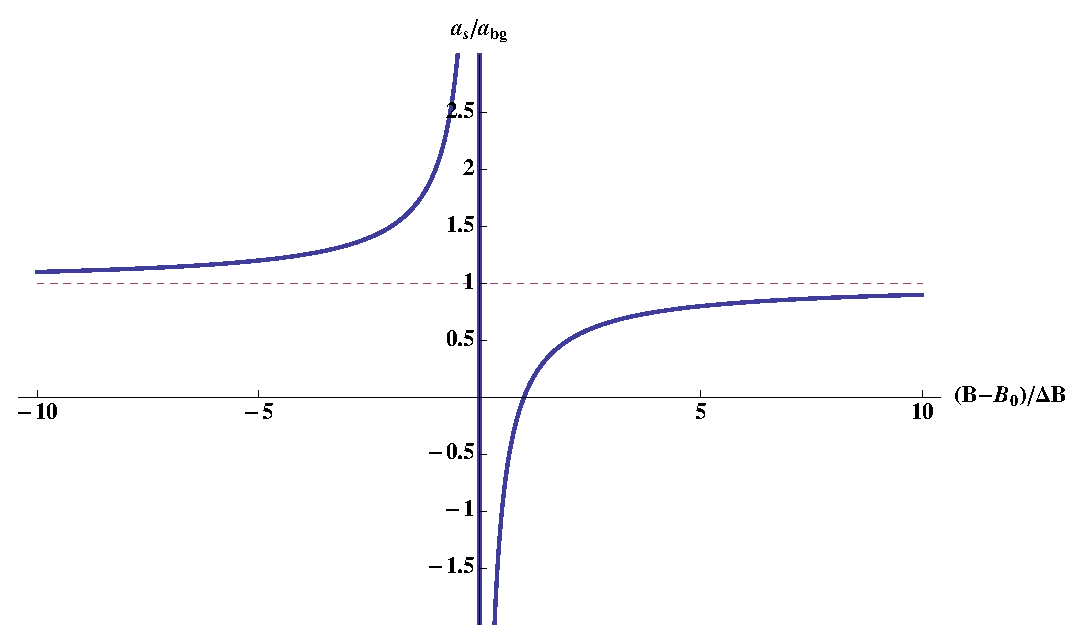
\includegraphics[width=0.6\textwidth]{FeshbachAs}
%\caption{S-wave scattering length in Feshbach resonance} 
\label{fig:intro:Feshbach}

\end{center}
\end{figure}
\end{itemize}

 }
 
 
 \frame{
 \frametitle{Potentials in a Feshbach resonance} 
  Channel: one  configuration of hyperfine spins for \myemph{one atom pair} in interaction, $|{F_{ }^{(1)},F_{z}^{(1)}}\rangle\otimes|{F_{ }^{(2)},F_{z}^{(2)}}\rangle$ 

\begin{figure}[htbp]
\begin{center}
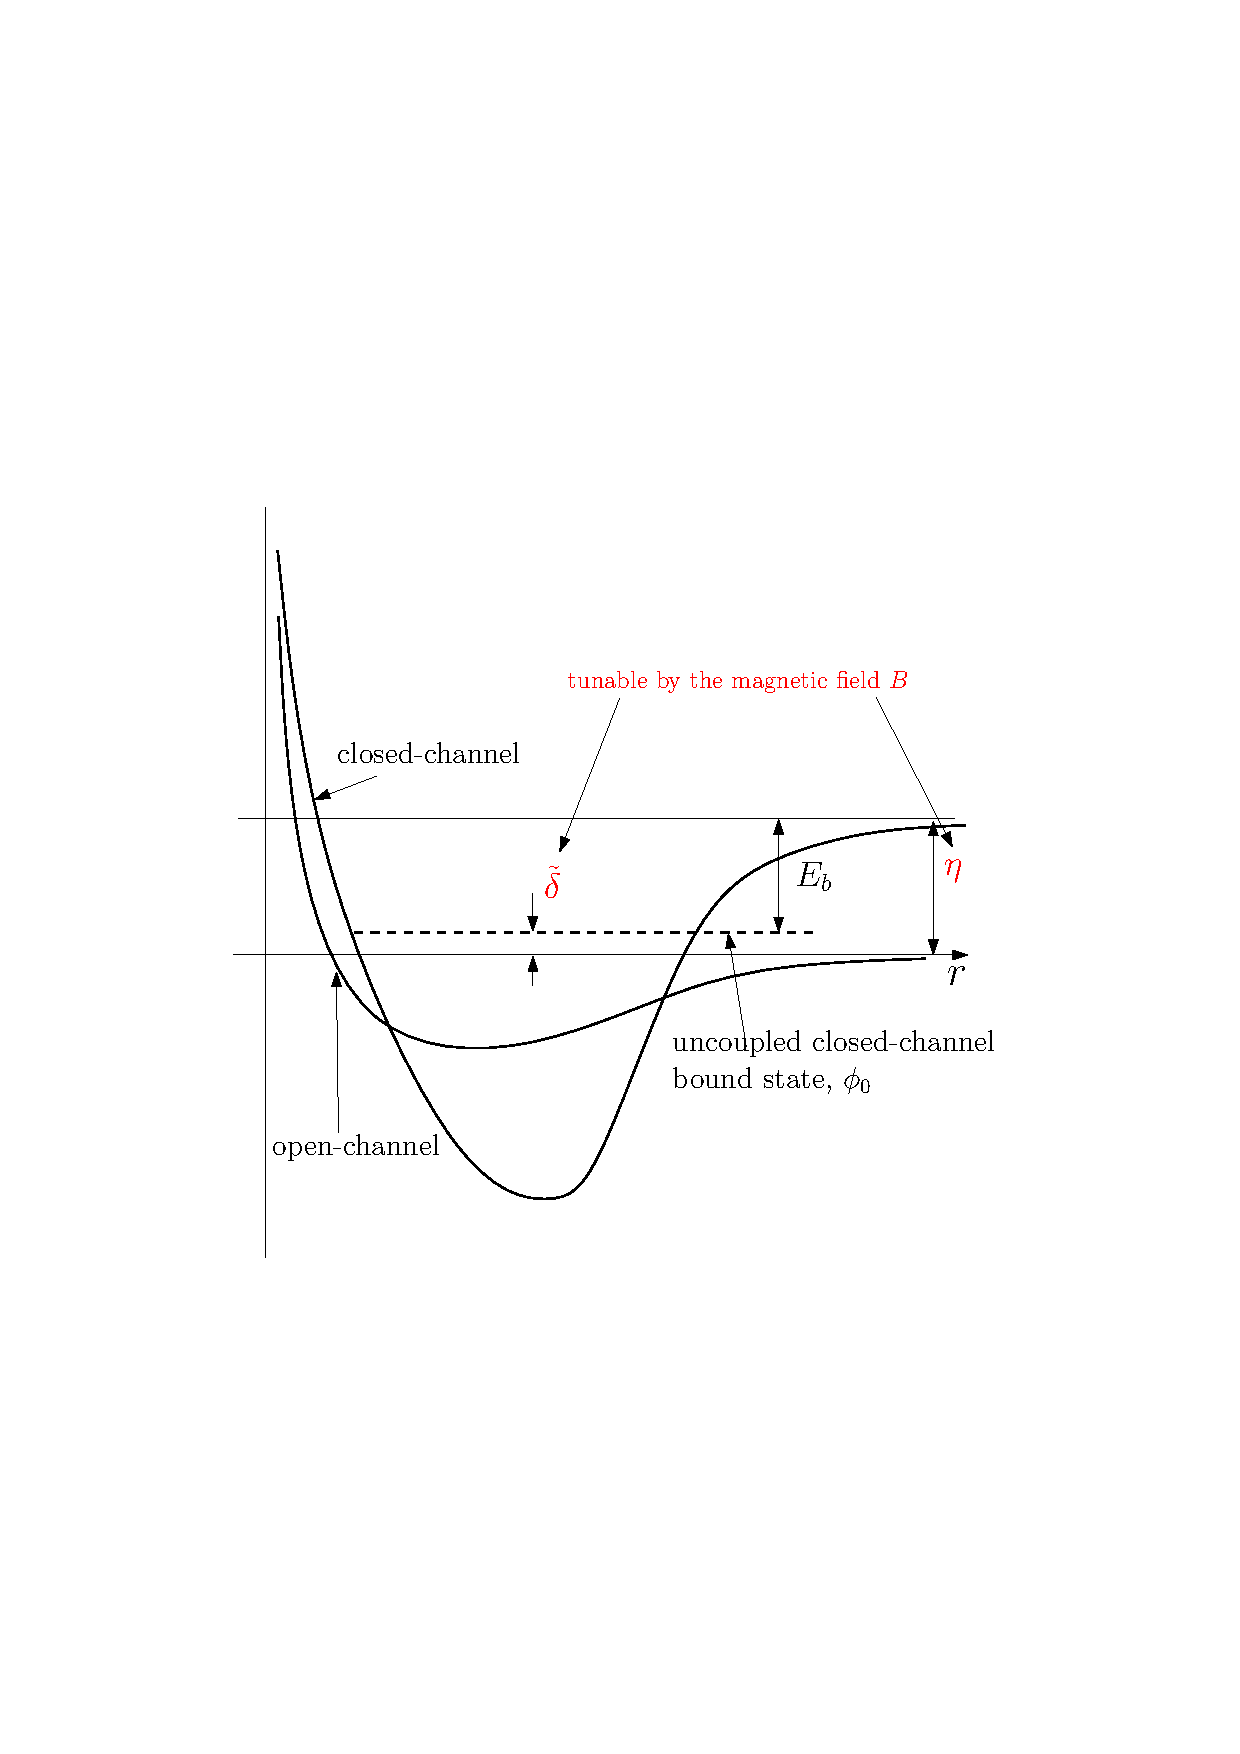
\includegraphics[width=0.8\textwidth]{2potential}

%Levels are marked with $F$ and $F_{z}$ {(see Footnote \ref{foot:intro:f} in page \pageref{foot:intro:f})} %Note that the energy of the $\ket{F=\nth{2},F_z=-\nth{2}}$ state first increases with the magnetic field, $B$, at low field then decrease at high field. In the same way, the energy of the $\ket{F=\frac{3}{2},F_z=-\nth{2}}$ state first decreases and then increases with the magnetic field.  
\label{fig:intro:li6}
\end{center}
\end{figure}
}


 \frame{
\frametitle{Scattering state and the bound state in a Feshbach resonance}
%\begin{columns}
%
%\begin{column}{0.6\textwidth}

\begin{figure}[htbp]
\begin{center}
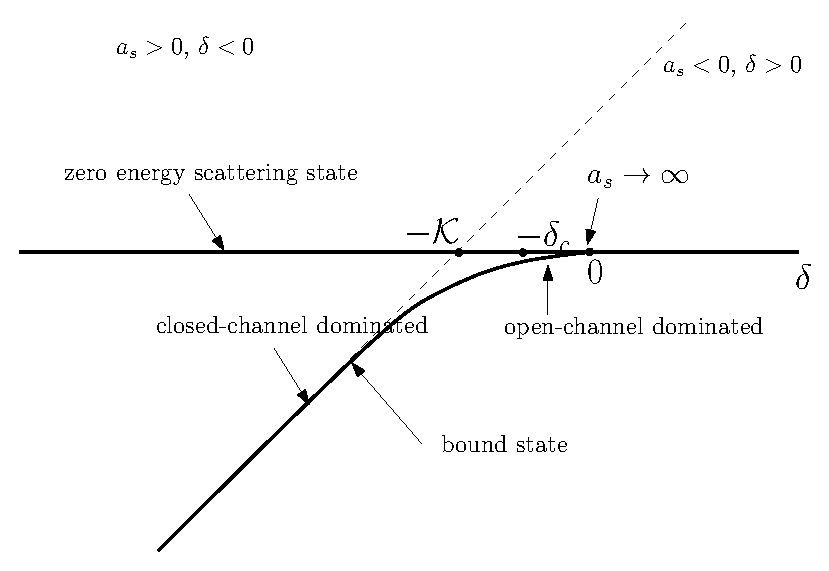
\includegraphics[width=0.6\textwidth]{levels}
%\caption{Energy levels in a Feshbach resonance\label{fig:intro:levels}} 
\end{center}
\end{figure}
Resonant point is not the level crossing point. The shift $\mathcal{K}$ is large than most energy scales.
$\delta=\tilde\delta-\mathcal{K}$

\pause
\begin{tabular}{|p{4cm}|p{4cm}|}
\hline
 $\mathemph{\abs{\delta}\ll\delta_{c}}$&$\mathemph{\abs{\delta}\gg\delta_{c}}$\\\hline
 Atoms are predominantly in the open-channel.&Atoms are predominantly in the closed-channel.\\
 \hline
\end{tabular}
%\end{column}
%\begin{column}{0.35\textwidth}

%\end{column}
%\end{columns}
}


\begin{frame}
\frametitle{Broad and narrow Feshbach resonance }

   \myemph{Many-body} introduce an important scale: 
         \myemph{ $E_F$}
         
 \pause
       \myemph{Broad resonance}: $\mathemph{\delta_c\gg{}E_F}$
        \begin{itemize}

\item The closed channel weight is negligible everywhere.
\item The closed channel is just like a simple knob for $a_{s}$
\item \myemph{The solutions of the single-channel model   applies.}
\item Most literatures  integrate the closed-channel out at broad resonance limit. 
\end{itemize}
   

              \pause
 
       \myemph{Narrow resonance}:  $\mathemph{\delta_c\ll{}E_F}$
        \begin{itemize}

\item The closed channel weight is substantial or even dominant close to the resonance.
\item \myemph{A two-channel  many-body model is necessary}. 
\item Studied by Gurarie and Radzihovsky \footnote{[Gurarie and Radzihovsky, Annals of Physics, 322(1):2 � 119.  2007]}
\end{itemize}
\end{frame}

\frame{
\frametitle{Three species problem}

\begin{itemize}
\item <1-> Two channels might share a \myemph{common} hyperfine species.
\item <2-> Interchannel Pauli exclusion between two channels.
\item <2->No counterpart in the two-body physics.  
\item <3->Only important in the narrow resonance. 
\item <3->No study on this subject in the literature. 
\item <1->Example: the resonance close to 834G in $^{6}$Li, 
\begin{itemize}
\item open-channel: $\ket{\frac{1}{2},-\nth{2}}\otimes\mathemph{\ket{\nth{2},+\nth{2}}}$;
\item closed-channel: $\ket{\frac{3}{2},-\nth{2}}\otimes\mathemph{\ket{\nth{2},+\nth{2}}}$.
\end{itemize}    It is a broad resonance though. 

\end{itemize}
}

\section[Single-channel]{Single-channel crossover}
\frame{
\frametitle{Single-channel crossover}
\begin{itemize}
\item  $\prod_{\vk}(u_{\vk}+v_{\vk}a^{\dg}_{\uparrow\vk}a^{\dg}_{\downarrow-\vk})\ket{0}=A\exp{}(\sum_{\vk}\frac{v_{\vk}}{u_{\vk}}a^{\dg}_{\uparrow\vk}a^{\dg}_{\downarrow-\vk})\ket{0}$
\item Continuously varying interactions ($a_{s}$)
\end{itemize}
\begin{figure}[htbp]
\begin{center}
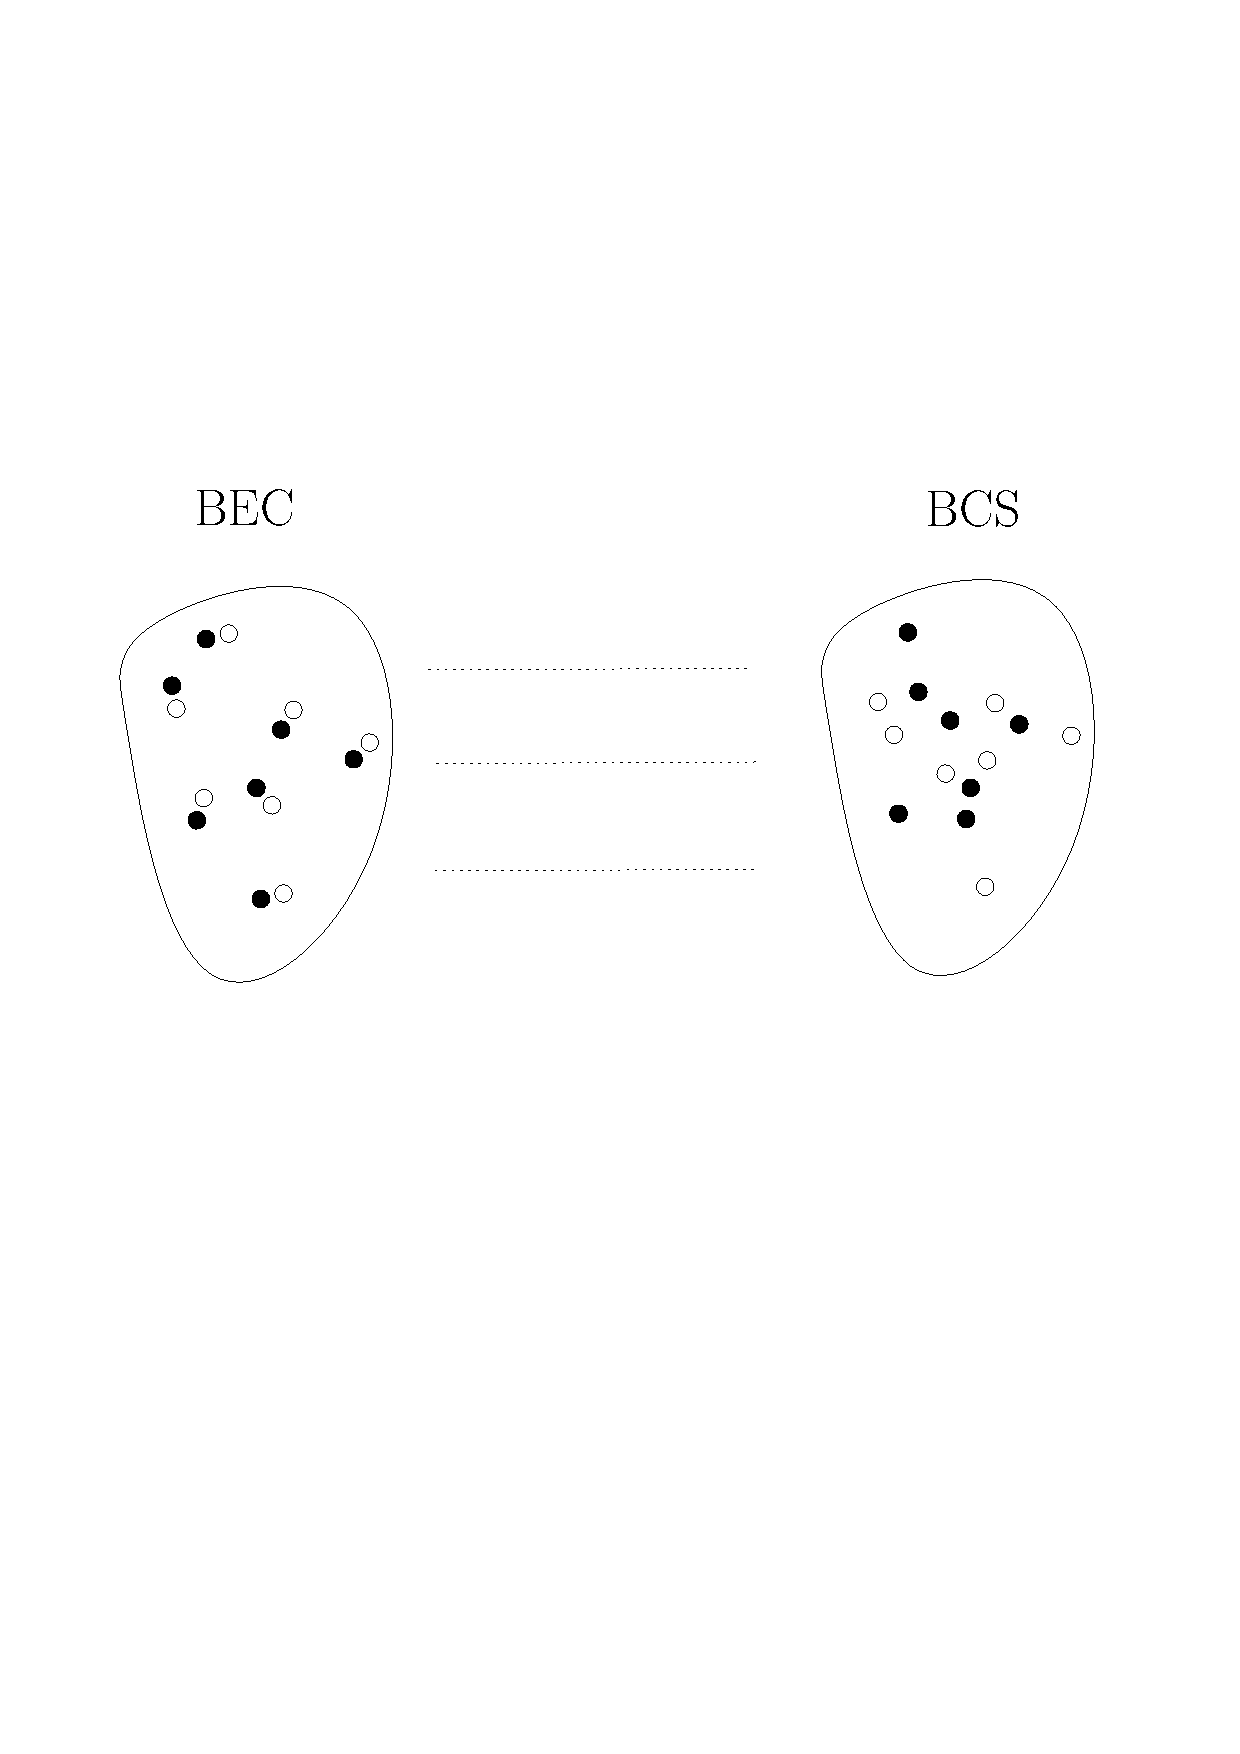
\includegraphics[width=0.7\textwidth]{crossover}
%\caption{Energy levels in a Feshbach resonance\label{fig:intro:levels}} 
\end{center}
\end{figure}
}
\frame{
\frametitle{The gap equation and the number equation}
 \myemph{The renormalized gap equation}
\begin{equation}\label{eq:pathInt:gapRenormalized}
\boxed{-\frac{m\mathcal{V}_{0}}{4\pi{}a_{s}}=\sum_{\vk}\mbr{\frac{1}{2E_k}-\nth{2\epsilon_{\vk}}}}
\end{equation}
$E_\vk=\sqrt{(\epsilon_\vk-\mu)^2+\abs{\Delta_0}^2}$;  $\mathcal{V}_0$: total volume.

\myemph{The number equation}
\begin{equation}
\boxed{N=\nth{\mathcal{V}_0}\sum_{\vk}\mbr{1-\frac{\epsilon_{\vk}}{E_{\vk}}}}
\end{equation}

}

\frame{
\frametitle{$\mu$ and $\Delta$ in the crossover}
\begin{figure}[htbp]
\begin{center}
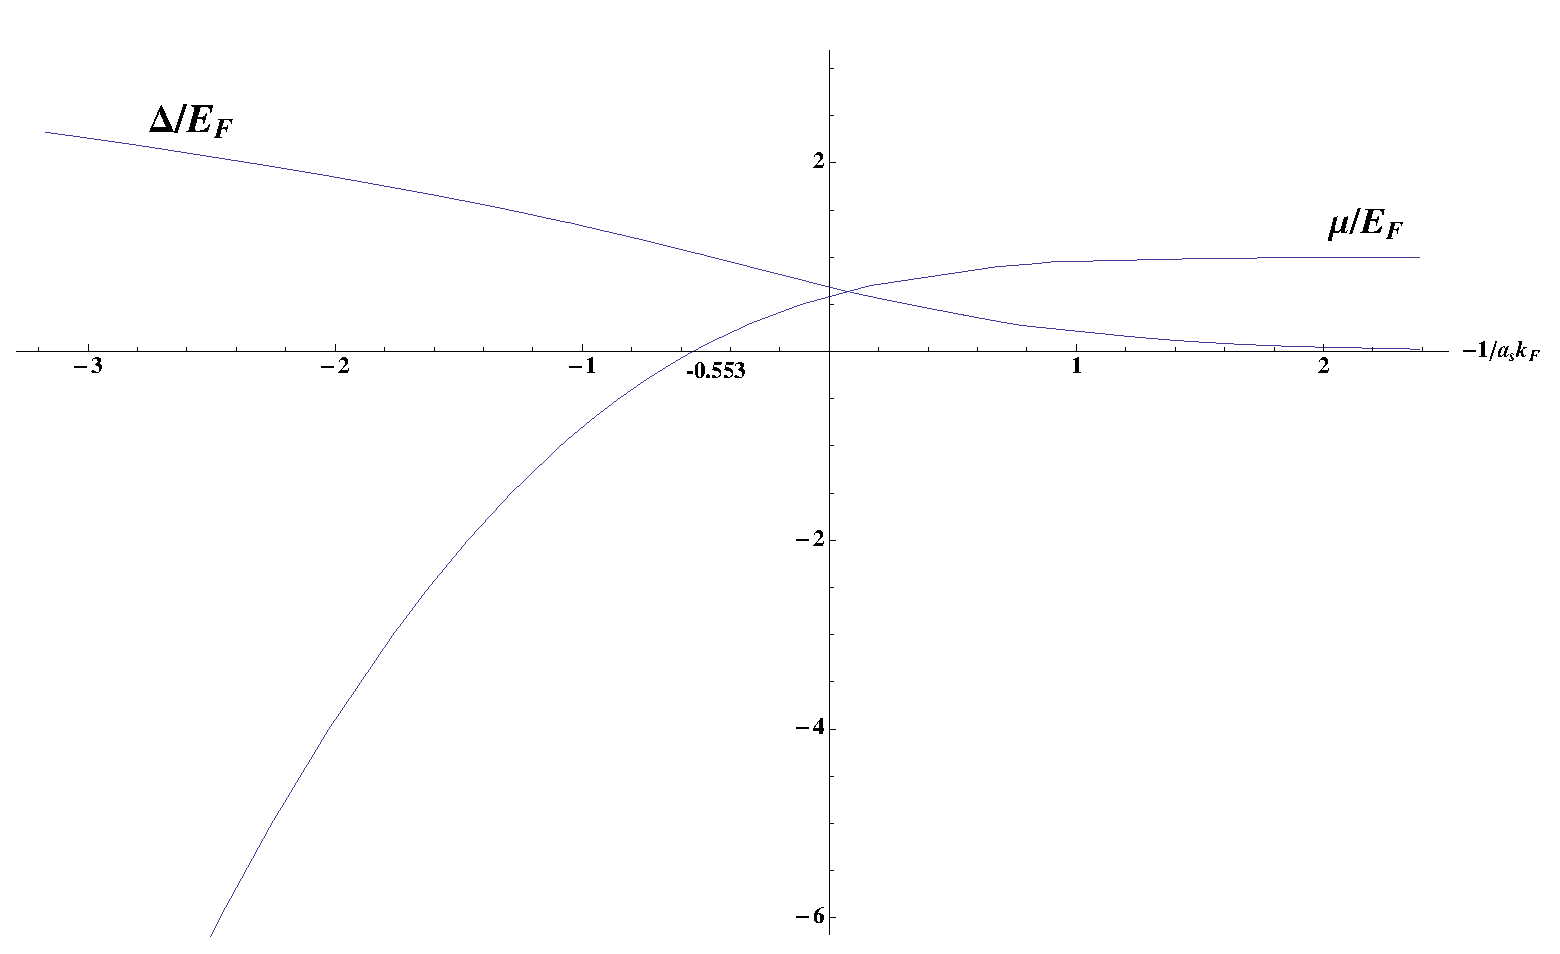
\includegraphics[width=0.8\textwidth]{SingleChannelCrossoverMuDelta}
\caption{The chemical potential $\mu$ and gap $\Delta$ in the mean field level over crossover} 
\label{fig:pathInt:meanField}
{\small All quantities in the unit of energy ($\mu$, $\Delta$) are rescaled with the Fermi energy $E_{F}$ and the s-wave scattering length $a_{s}$ is rescaled with $1/k_{F}$.  }
\end{center}
\end{figure}
}


\section[Two-channel]{Two-channel three-species crossover model}

\frame{
\frametitle{Extremely narrow resonance}
The coupling between two channels is assumed to be extremely weak ($Y\to0$). $\mathcal{K}\to0$, $\delta_{c}\to0$. Infinitely narrow resonance.  Two channels share the same chemical potentials. 
\begin{figure}[hhtb]
	\centering
	         \subfloat[$E_{F}<\tilde\delta$]{\label{fig:narrowFR:aboveSea}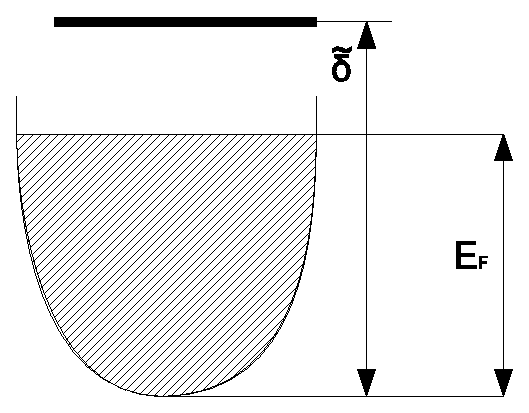
\includegraphics[width=.2\textwidth]{narrowFRabove.eps}}\quad
		\subfloat[$0<\tilde\delta<E_{F}$]{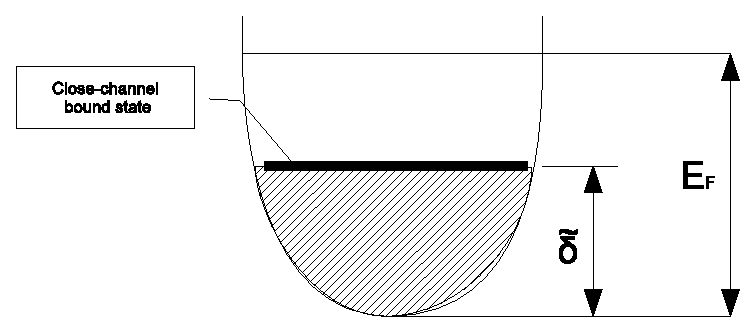
\includegraphics[width=.30\textwidth]{narrowFRin.eps}\label{fig:narrowFR:inSea}}\quad
		\subfloat[$\tilde\delta<0$]{\label{fig:narrowFR:belowSea}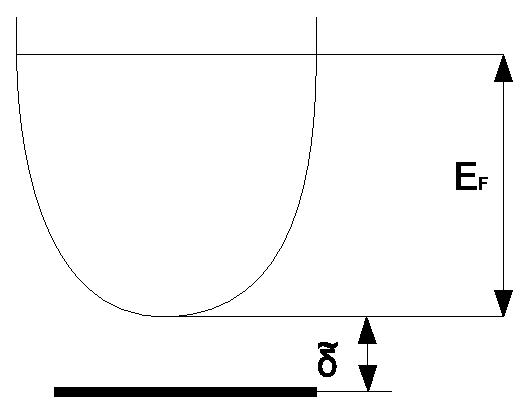
\includegraphics[width=.20\textwidth]{narrowFRbelow.eps}}
	%\caption{Extremely narrow resonance\label{fig:narrowFR}}
	%\small{The shaded area is occupied by atoms. }
	%\parbox{0.7\textwidth}{\small{  In Fig. \subref{fig:narrowFR:inSea} chemical potential would be close to the closed-channel bound state level (besides small shift due to the open-channel intra-channel coupling) and the ``Fermi sea'' above is empty. }}
\end{figure}
\begin{itemize}
\item Energy is counted from Fermi surface;
\item Atoms distributed in both channels in (b); 
\item The inter-channel Pauli exclusion persists in (b).
\end{itemize}
}

\frame{
\frametitle{Interchannel Pauli exclusion: handwave discussion}
\begin{itemize}[<+->]
\item Determined by the overlap between two channels
\item One simplification: \myemph{the uncoupled closed-channel bound state, $\phi_{0}$, is much smaller than the interparticle distance in size}. 
\item Size of $\phi_{0}$ in the closed-channel: $\sim{E_{b}}^{-1/2}$
\item Size of atoms in the open-channel: interparticle distance $a_{0}\sim{}E_{F}^{-1/2}$
\item Controlling parameter
\begin{equation}\label{eq:pathInt2:zetaDef}
\boxed{\zeta=\frac{\Delta_{2}^{2}}{\Delta_{1}\eta}\sim\br{\frac{E_{F}}{E_{b}}}^{1/2}\ll1}
\end{equation}
\item Small $\zeta$ dictates a \myemph{perturbative} treatment. 
\end{itemize}
}

\frame{
\frametitle{Hamiltonian and Hubbard-Strotonovich trans.}
\begin{equation}
\begin{split}\label{eq:pathInt2:actionFermi}
&S(\bar\psi,\psi)=\int^{\beta}_{0}d\tau\int{d^{d}r}\\
&\Big[\sum_{j}\bar\psi_{j}(\partial_\tau-\nth{2m}\nabla^{2}-\mu+\eta_{j})\psi_{j}
-(\bar\psi\bar\psi)\tilde{U}(\psi\psi)\Big]
\end{split}
\end{equation}
Hubbard-Strotonovich transformation: introduce a two-component auxiliary field (order parameters)
\begin{equation*}
\mtrx{\Delta_{1}\\\Delta_{2}}\longrightarrow
	\mtrx{\Delta_{1}\\\Delta_{2}}-
	\mtrx{U&Y\\Y^{*}&V}
	\mtrx{\psi_{b}\psi_{a}\\\psi_{c}\psi_{a}}
\end{equation*}\pause
The action can then be rewritten in a more compact form with respect to $\Psi$ and $\bar\Psi$
\begin{equation}\label{eq:pathInt2:actionMixCompact}
S(\bar\Delta,\Delta,\bar\psi_{i},\psi_{i})=\int^{\beta}_{0}d\tau\int{d^{d}r}
	\mbr{\Delta^{\dg}\tilde{U}^{-1}\Delta-\bar\Psi\mathcal{G}^{-1}\Psi}
\end{equation}
%It is bilinear of $\Psi$.  We can integrate it out,
%\begin{equation}\label{eq:pathInt2:actionD}
%S(\bar{\Delta},\Delta)=\int{dx}\br{\bar{\Delta}\tilde{U}^{-1}\Delta-\tr\ln\nG}
%\end{equation}



}
\note{$\Delta_{1}$  $\Delta_{2}$ do not correspond to open-/closed-channel.}

\frame{
\frametitle{Mean-field equations}
 Integrate out $\psi_{i}$
\begin{equation}\label{eq:pathInt2:actionD}
S(\bar{\Delta},\Delta)=\int{dx}\br{\bar{\Delta}\tilde{U}^{-1}\Delta-\tr\ln\nG}
\end{equation}
Mean field equation:

  \begin{equation}\label{eq:pathInt2:mf}
\mtrx{\Delta_1\\\Delta_2}=\mtrx{U&Y\\Y^{*}&V}\sum_{\vk}\mtrx{h_{1\vk}\\h_{2\vk}}
\end{equation}
  where 
  \begin{gather}
  h_{1\vk}=\av{\psi_{a,-{\vk}}\psi_{b,+{\vk}}}
  =\Delta_{1}\frac{E_{1\,\vk}+\xi_{\vk}+\eta}{(E_{1\,\vk}+E_{2\,\vk})(E_{1\,\vk}+E_{3\,\vk})}\label{eq:pathInt2:h1}\\
  h_{2\vk}=\av{\psi_{a,-{\vk}}\psi_{c,+{\vk}}}
  =\Delta_{2}\frac{E_{1\,\vk}+\xi_{\vk}}{(E_{1\,\vk}+E_{2\,\vk})(E_{1\,\vk}+E_{3\,\vk})}\label{eq:pathInt2:h2}
  \end{gather}

}
\frame{
\frametitle{Order parameters}
\begin{itemize}

\item Gor'kov Green function for $\bar\Psi=\mtrx{\bar\psi_{a}&\psi_{b}&\psi_{c}}$, fermionic correlation
\begin{equation}\label{eq:pathInt2:nGDeltaK}
\mathcal{G}^{-1}=
\begin{pmatrix}
i\omega_{n}-\xi_{k}&\Delta_{1}&{\mathemph{\Delta_{2}}}\\
\bar\Delta_{1}&i\omega_{n}+\xi_{k}&0\\
\mathemph{\bar\Delta_{2}}&0&i\omega_{n}+\xi_{k}+\eta
\end{pmatrix}
\end{equation}
\item $\Delta_{1}$ includes the coupling with the closed-channel, $Y$; 

\item $\mathemph{\Delta_2}$ terms describe the inter-channel Pauli exclusion. 
\pause
\item Solved the three-species two-channel problem in two steps:
\begin{enumerate}
\item Treat effects other than the inter-channel Pauli exclusion in a non-perturbative way; ($\mathemph{\Delta_2=0}$)
\item Treat the inter-channel Pauli exclusion perturbavtively. 

\end{enumerate}
\end{itemize}

}

%\frame{
%\frametitle{Two-channel three-species model}
%\begin{itemize}
%\item Two order parameters 
% \begin{equation}\label{eq:pathInt2:mf}
%\mtrx{\Delta_1\\\Delta_2}=\mtrx{U&Y\\Y^{*}&V}\sum_{\vk}\mtrx{<{\psi_{a,-{\vk}}\psi_{b,+{\vk}}}>\\<{\psi_{a,-{\vk}}\psi_{c,+{\vk}}}>}
%\end{equation}
%\item Order parameters are result of mixed channel;
%\item $\Delta_{1}$ corresponds to the single channel gap;
%\item $\Delta_{1}$ includes the broad resonance limit effect (the $Y$ coupling with the closed-channel); 
%\item Reduced to the single-channel by two steps:
%\begin{enumerate}
%\item Treat effects other than the inter-channel Pauli exclusion in a non-perturbative way;
%\item Treat the inter-channel Pauli exclusion perturbavtively. 
%\end{enumerate}
%\end{itemize}
%}


\frame{
	\frametitle{Narrow resonance w/o interchannel Pauli exclusion}
	
	\begin{itemize}
\item Energy zero moves to the Fermi surface
\begin{gather}
1=-\mbr{\frac{4\pi{\mathemph{\tilde{a}_{s}}(\mu)}}{m}\sum(\nth{2E_{\vk}}-\nth{2\epsilon_{\vk}})}\label{eq:pathInt2:narrowGapS}\\
\tilde{a}_{s}=a_{\text{bg}}(1+\frac{\mathcal{K}}{\delta-\mathemph{2\mu}})\approx{}\frac{a_{\text{bg}}\mathcal{K}}{\delta-\mathemph{2\mu}}
\end{gather}
\item Extra counting for the closed-channel. 
\begin{gather}
\mathemph{N_{\text{open}}}=\sum_\vk\mbr{1-\frac{\epsilon_{\vk}}{E_{\vk}}}\label{eq:pathInt2:narrowNumS}
\end{gather}
\item  Consistent with  the study by Gurarie and Radzihovsky \footnote{[Gurarie and Radzihovsky, Annals of Physics, 322(1):2 � 119.  2007]}
\end{itemize}
}
\frame{
\frametitle{Narrow resonance w/o interchannel Pauli exclusion}
\begin{figure}[htbp]
\begin{center}
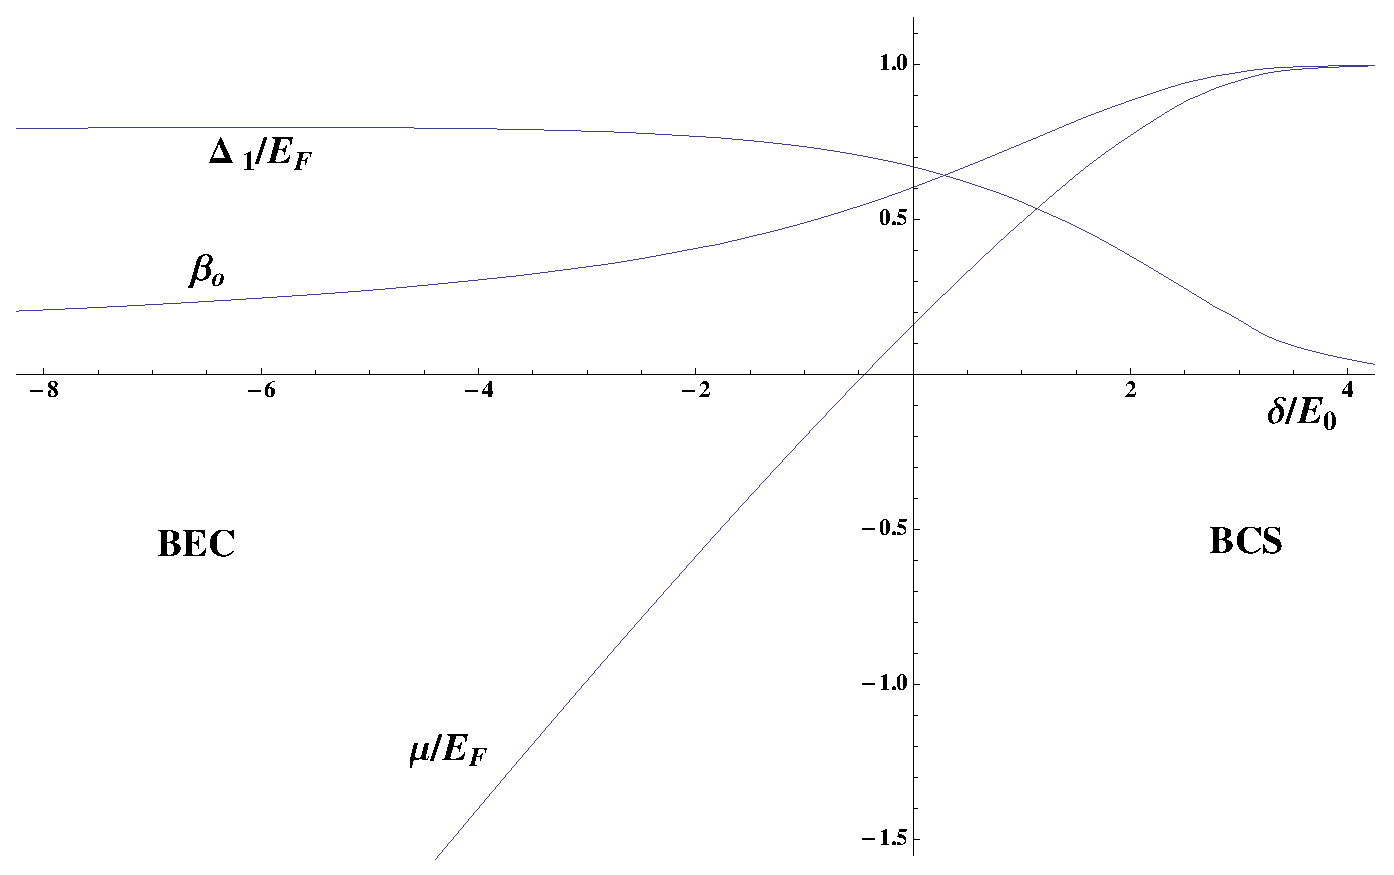
\includegraphics[width=0.8\textwidth]{narrow}
%\caption{The chemical potential $\mu$, the open-channel gap $\Delta_{1}$ and the open-channel relative weight $\beta_{o}$ over crossover with the narrow Feshbach resonance without considering the inter-channel Pauli exclusion  vs. the chemical potential and the gap in the single-channel model} 
\label{fig:pathInt2:narrow}
%{\small  The gap in the open-channel $\Delta_{1}$ and the chemical potential $\mu$ are rescaled with the the Fermi energy of the total density, $E_{F}^{(tot)}$.  The $x$-axis is the detuning $\delta$ rescaled with $E_{0}$ (see Eq. \ref{eq:pathInt2:E0}) for the narrow resonance; while it is $-1/a_{s}k_{F}$ for the single-channel curves. We have taken $\delta_{c}=0.001E_{F}^{(tot)}$ for the narrow resonance figure. We used the detuning from the resonant point  for the $x$-axis in the narrow resonance instead of $-1/a_{s}k_{F}$ in the single-channel because the additional shift, $2\mu$, considering in Eq. \ref{eq:pathInt2:simplenarrowAs}.  Consequently, the chemical potential lines in both cases cross the $x$-axis at the same point where $\mu=0$.  }
\end{center}
\end{figure}
\begin{itemize}
\item $\Delta_{1}$ saturates in BEC side
\item $\tilde{a}_{s}$ differs from two-body $a_{s}$ with special shift $2\mu$
\item $\beta_{o}=\frac{n_{open}}{n_{total}}$ deviates from 1 substantially at universality

\end{itemize}
}




\frame{
\frametitle{Fermionic modes}
Diagonalize Gor'kov Greens function
\begin{columns}
\column{0.55\textwidth}
\begin{align*}
E_{1\vk}&\approx{}E_{\vk}+\mathemph{u_{\vk}^{2}\Delta_{1}\zeta}\\
E_{2\vk}&\approx{}E_{\vk}-\mathemph{v_{\vk}^{2}\Delta_{1}\zeta}\\
E_{3\vk}&\approx{}\epsilon_{\vk}+\eta+\mathemph{\frac{\zeta}{2}\Delta_{1}}
\end{align*}
\column{0.45\textwidth}
\begin{equation*}
\boxed{\zeta=\frac{\Delta_{2}^{2}}{\Delta_{1}\eta}}
\end{equation*}
$E_\vk=\sqrt{(\epsilon_\vk-\mu)^2+\abs{\Delta_1}^2}$
\end{columns}
\begin{itemize}
\item $E_{1\vk}$ and $E_{2\vk}$ are like Bogoliubov quasi-paticle; 
\item $E_{1\vk}$ and $E_{2\vk}$ now split by $\Delta_1\zeta$;
\item $E_{3\vk}$ is the free fermionic excitation in the close-channel;
\pause
\item The correction is in the order of $\zeta\ll1$;
\item The correction is due to the inter-channel Pauli exclusion and does not disappear even at the extremely narrow limit. 
\end{itemize}

}



\frame{
\frametitle{Bosonic modes}
Fluctuations of the order parameters;
\begin{itemize}
\item<1-> Order parameters describe the collective properties of atoms;
\item<2-> Four possible modes for two complex order parameters ($\Delta_1$, $\Delta_2$);
\item<3-> The overall phase fluctuation mode is the Goldstone mode;
\item<3-> The other three modes are massive;
\item<4-> The inter-channel out-of-sync phase mode is gapped at pair-breaking energy;
\item<5-> Corrections due to the inter-channel Pauli exclusion is in the order of $\zeta$.
\end{itemize}
}

\section{Discussion}
\frame{
\frametitle{Discussion}
\begin{itemize}
\item<1-> The inter-channel Pauli exclusion can be handled by perturbation method;
\item<1-> Handling two-channel problem, especially the inter-channel Pauli exclusion effect, self-consistently;
\item<2-> Using the BCS-approach (non-perturbative) as the zeroth order, building narrow resonance with the  inter-channel Pauli exclusion upon it;
\item<2-> The methodology about narrow resonance is still valid for non-simple-BCS treatment about crossover;

\item<3-> Finite temperature: BCS $\Rightarrow$ Fermi liquid; BEC $\Rightarrow$ normal dimer gas.  
\end{itemize}
}
\frame{
\begin{center}
 \Huge Thank you!
\end{center}

}
\end{document}


\section{Conclusion}
\frame{}
\bibliography{../citation}
\bibliographystyle{plain}
%\bibliographystyle{apalike}
\end{document}
